\documentclass{beamer}
%\documentclass[handout,t]{beamer}
\newcommand{\btVFill}{\vskip0pt plus 1filll}

\batchmode
% \usepackage{pgfpages}
% \pgfpagesuselayout{4 on 1}[letterpaper,landscape,border shrink=5mm]

\usepackage{amsmath,amssymb,enumerate,epsfig,bbm,calc,color,ifthen,capt-of}

\usetheme{Berlin}
\usecolortheme{bear}

\title{Combinatorial and Geometric Structure in the Self-Assembly of Polyhedra}
\author{Daniel Johnson}
%\date{\today}
\date{April 15, 2015}
%\date{March 26, 2015}
\pgfdeclareimage[height=1cm]{brown-logo}{brown-logo.pdf}
\logo{\pgfuseimage{brown-logo}\hspace*{0.3cm}}

\AtBeginSection[]
{
  \begin{frame}<beamer>
    \frametitle{Outline}
    \tableofcontents[currentsection]
  \end{frame}
}
\beamerdefaultoverlayspecification{<+->}
% -----------------------------------------------------------------------------
\begin{document}
% -----------------------------------------------------------------------------

\frame{\titlepage}

\section[Outline]{}
\begin{frame}{Outline}
  \tableofcontents
\end{frame}
% -----------------------------------------------------------------------------
% -----------------------------------------------------------------------------
\section{Introduction}
%\subsection{Polyhedra}
\begin{frame}{Platonic Solids}
\begin{itemize}
  \item Composed of a single type of regular polygon
  \item 5 Platonic Solids
\end{itemize}
\vspace{0.1 in}
\begin{columns}
    \begin{column}{0.32\textwidth}
      \centering
      %Cube

      \scalebox{0.035}{
        \begin{figure}
          \centering
          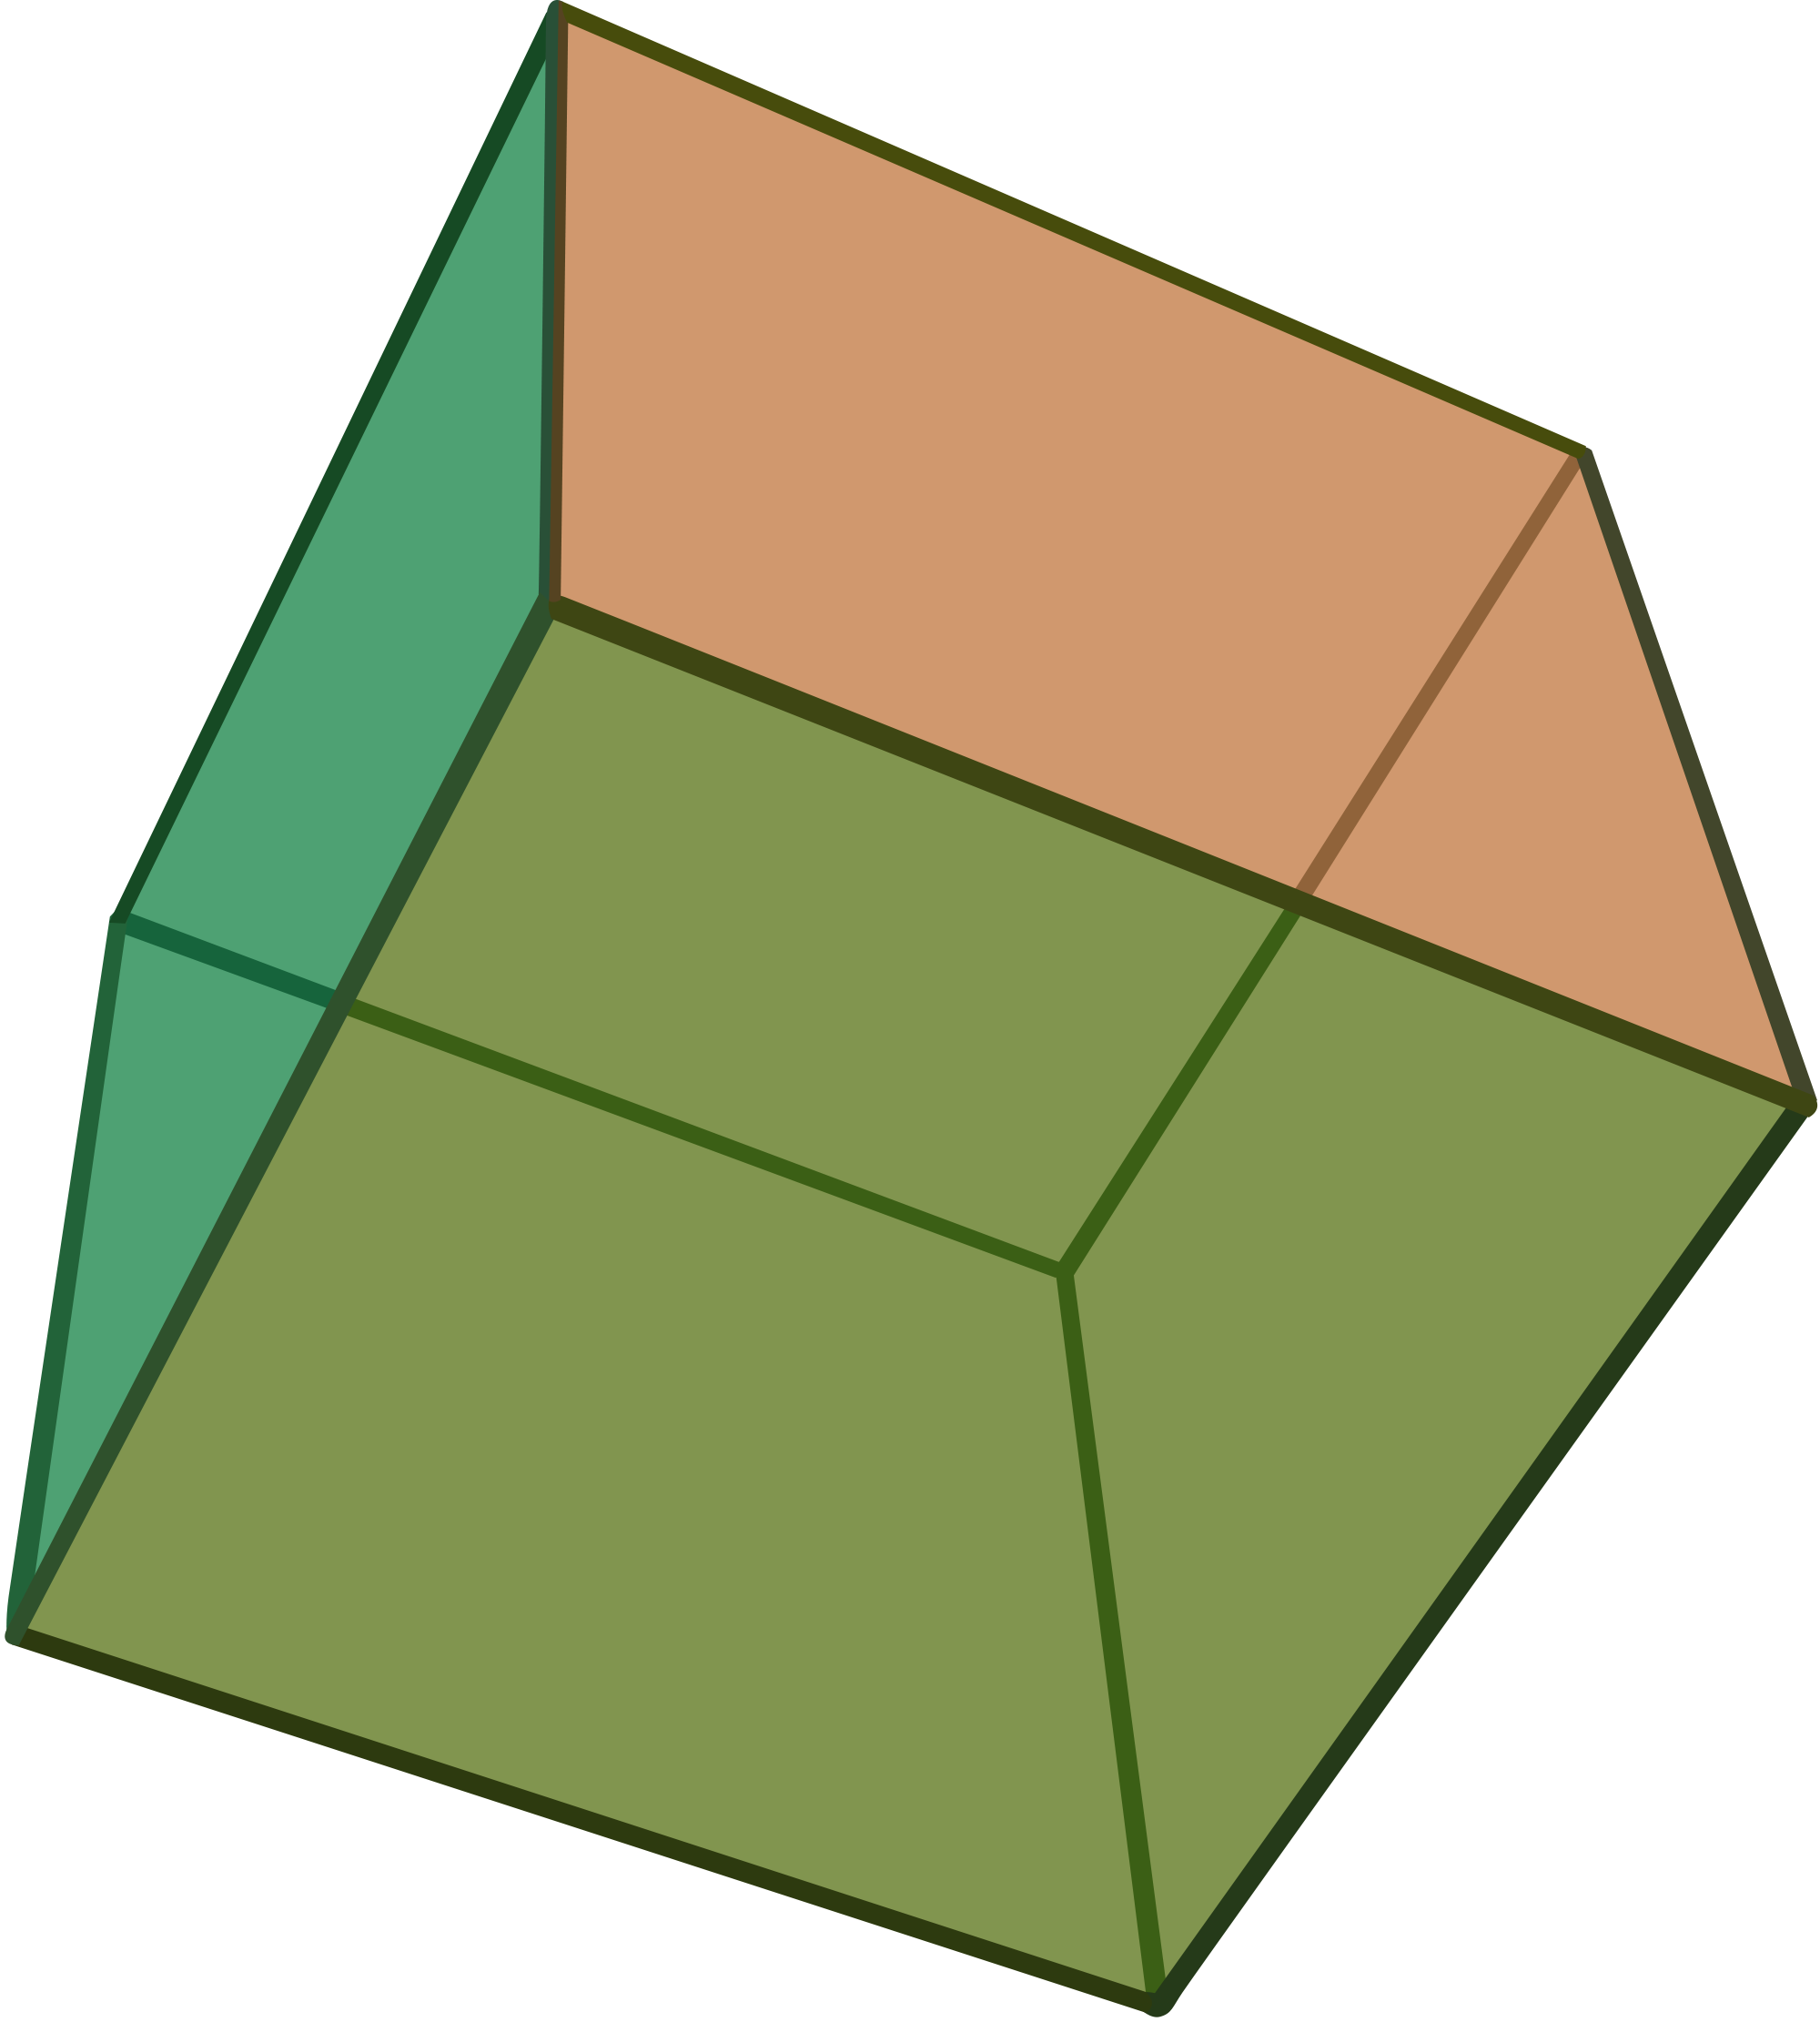
\includegraphics{cube.png}
        \end{figure}
      }

      Cube
     \end{column}
    \begin{column}{0.32\textwidth}
      \centering
      %Octahedron
      
      \scalebox{0.035}{
        \begin{figure}
          \centering
          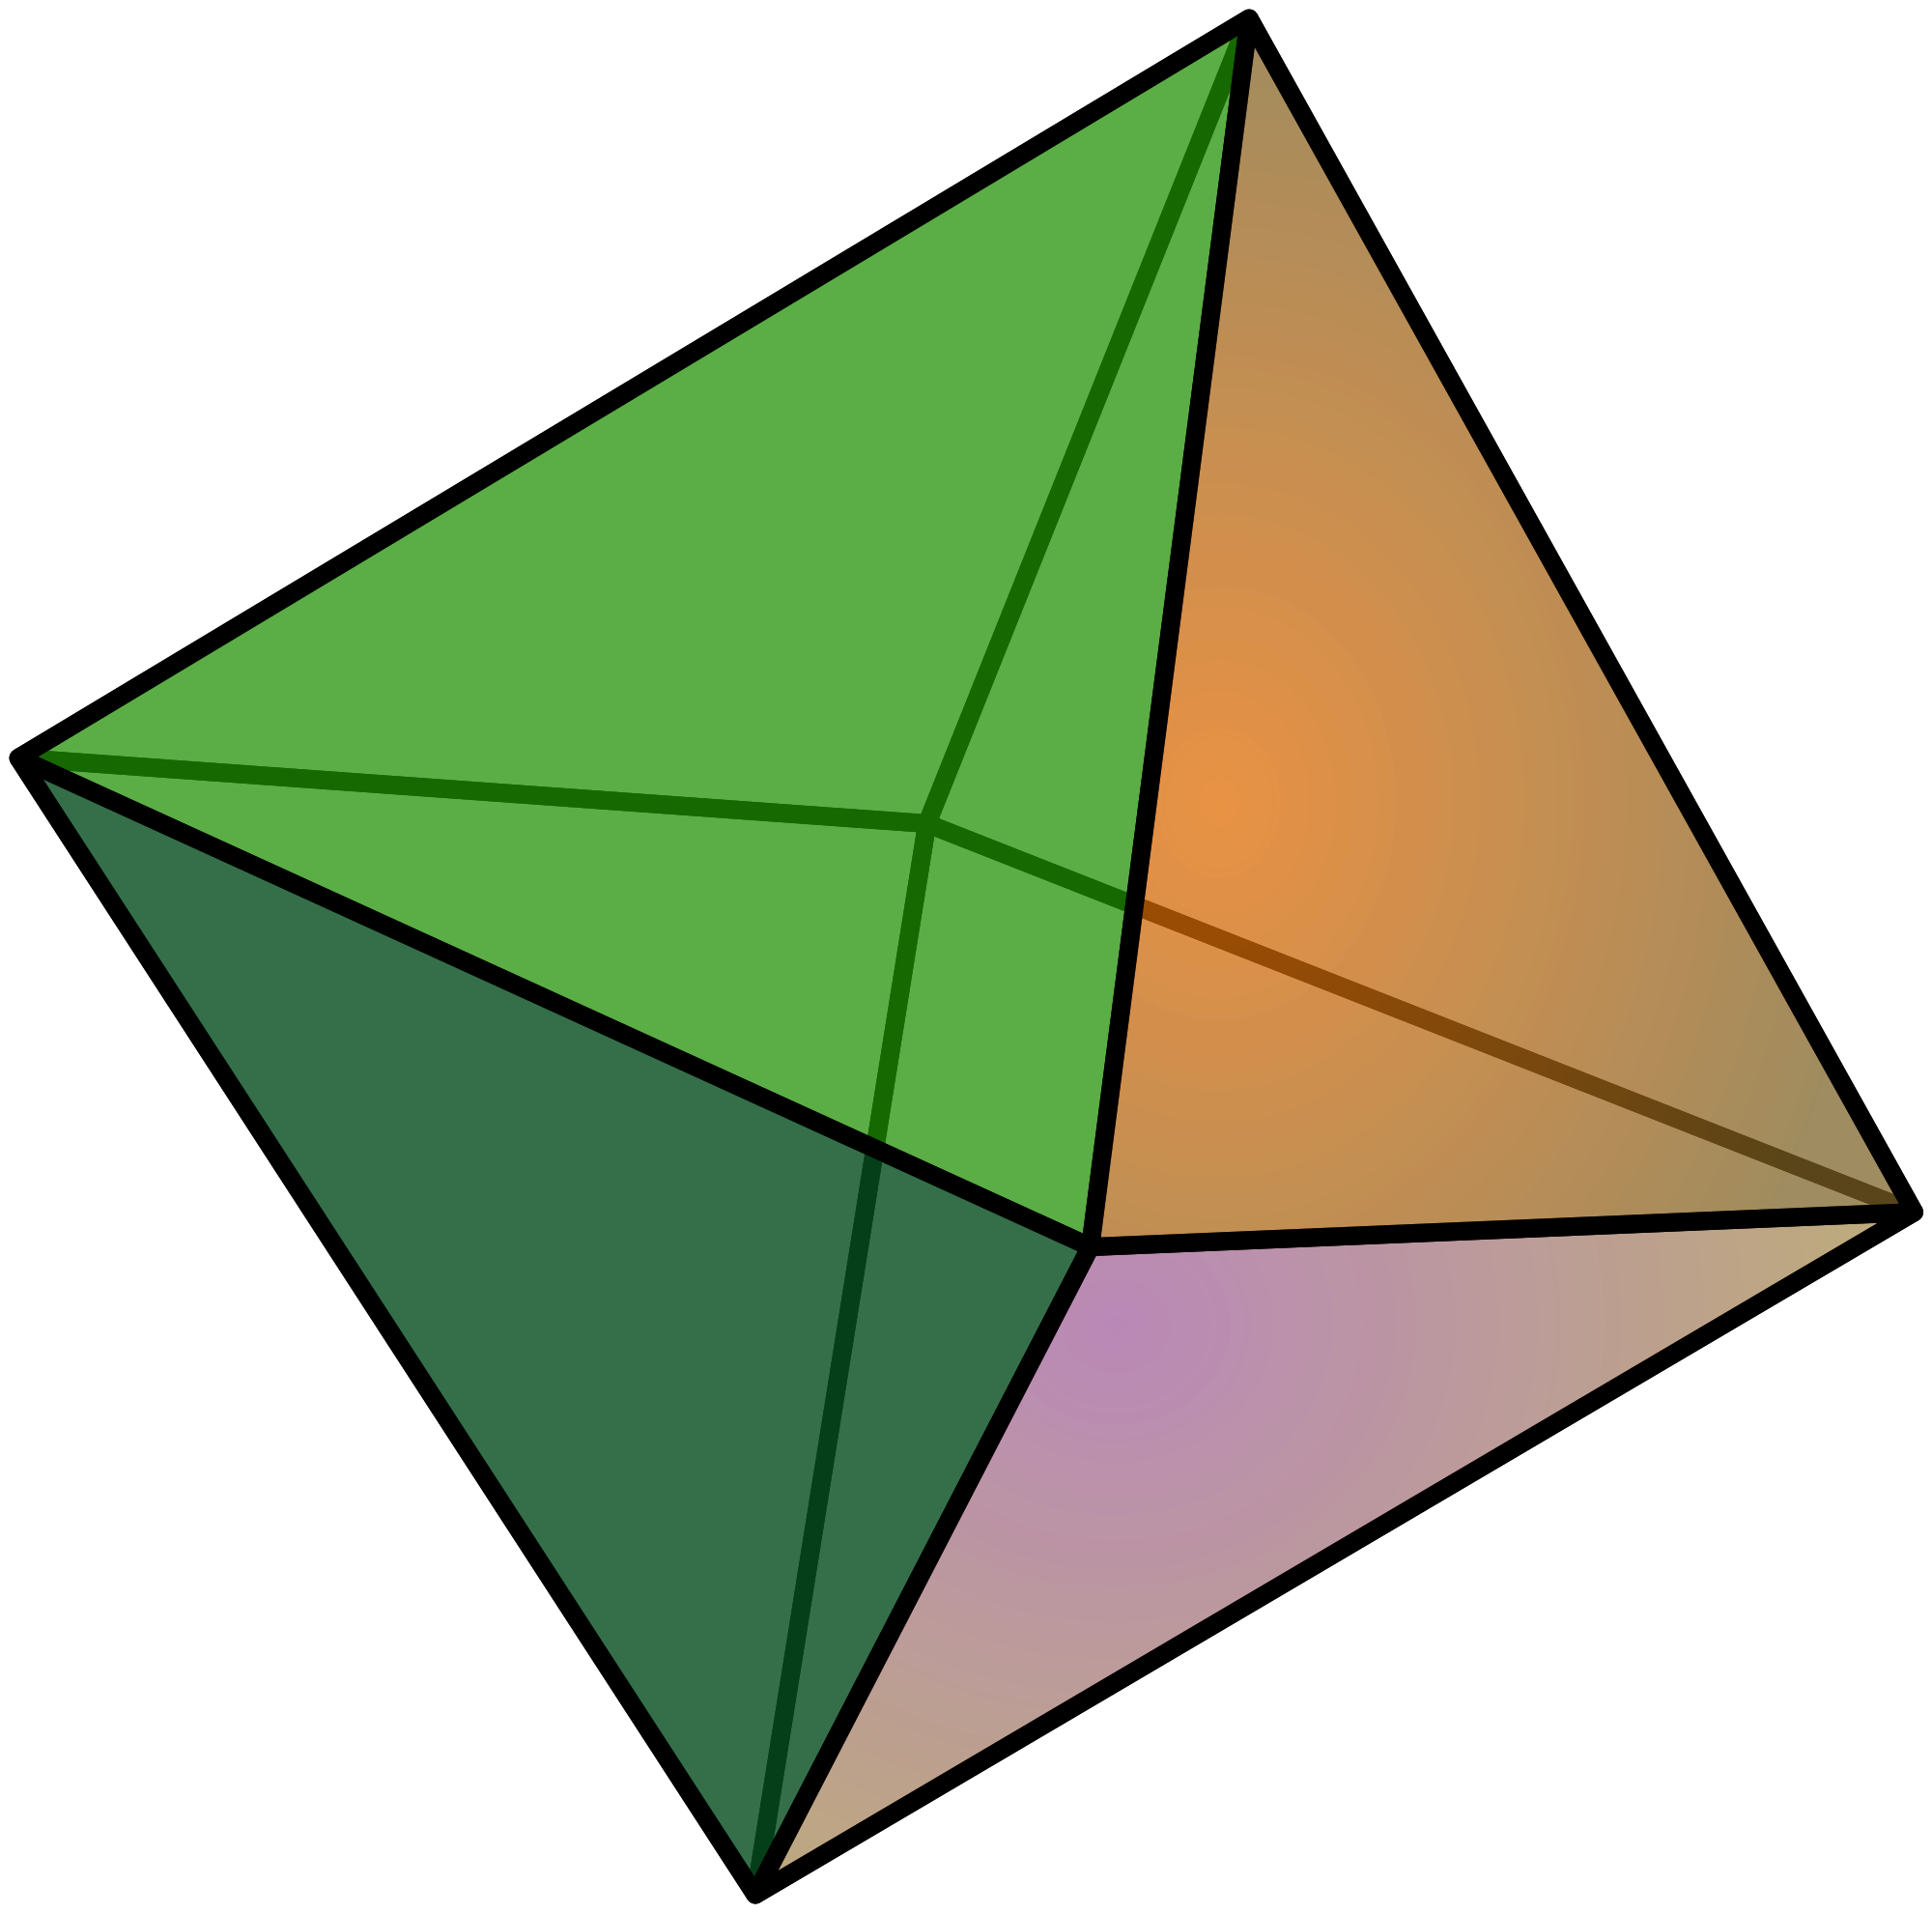
\includegraphics{octahedron.png}
        \end{figure}
      }

      Octahedron
     \end{column}
    \begin{column}{0.32\textwidth}
      \centering
      
      \scalebox{0.035}{
        \begin{figure}
          \centering
          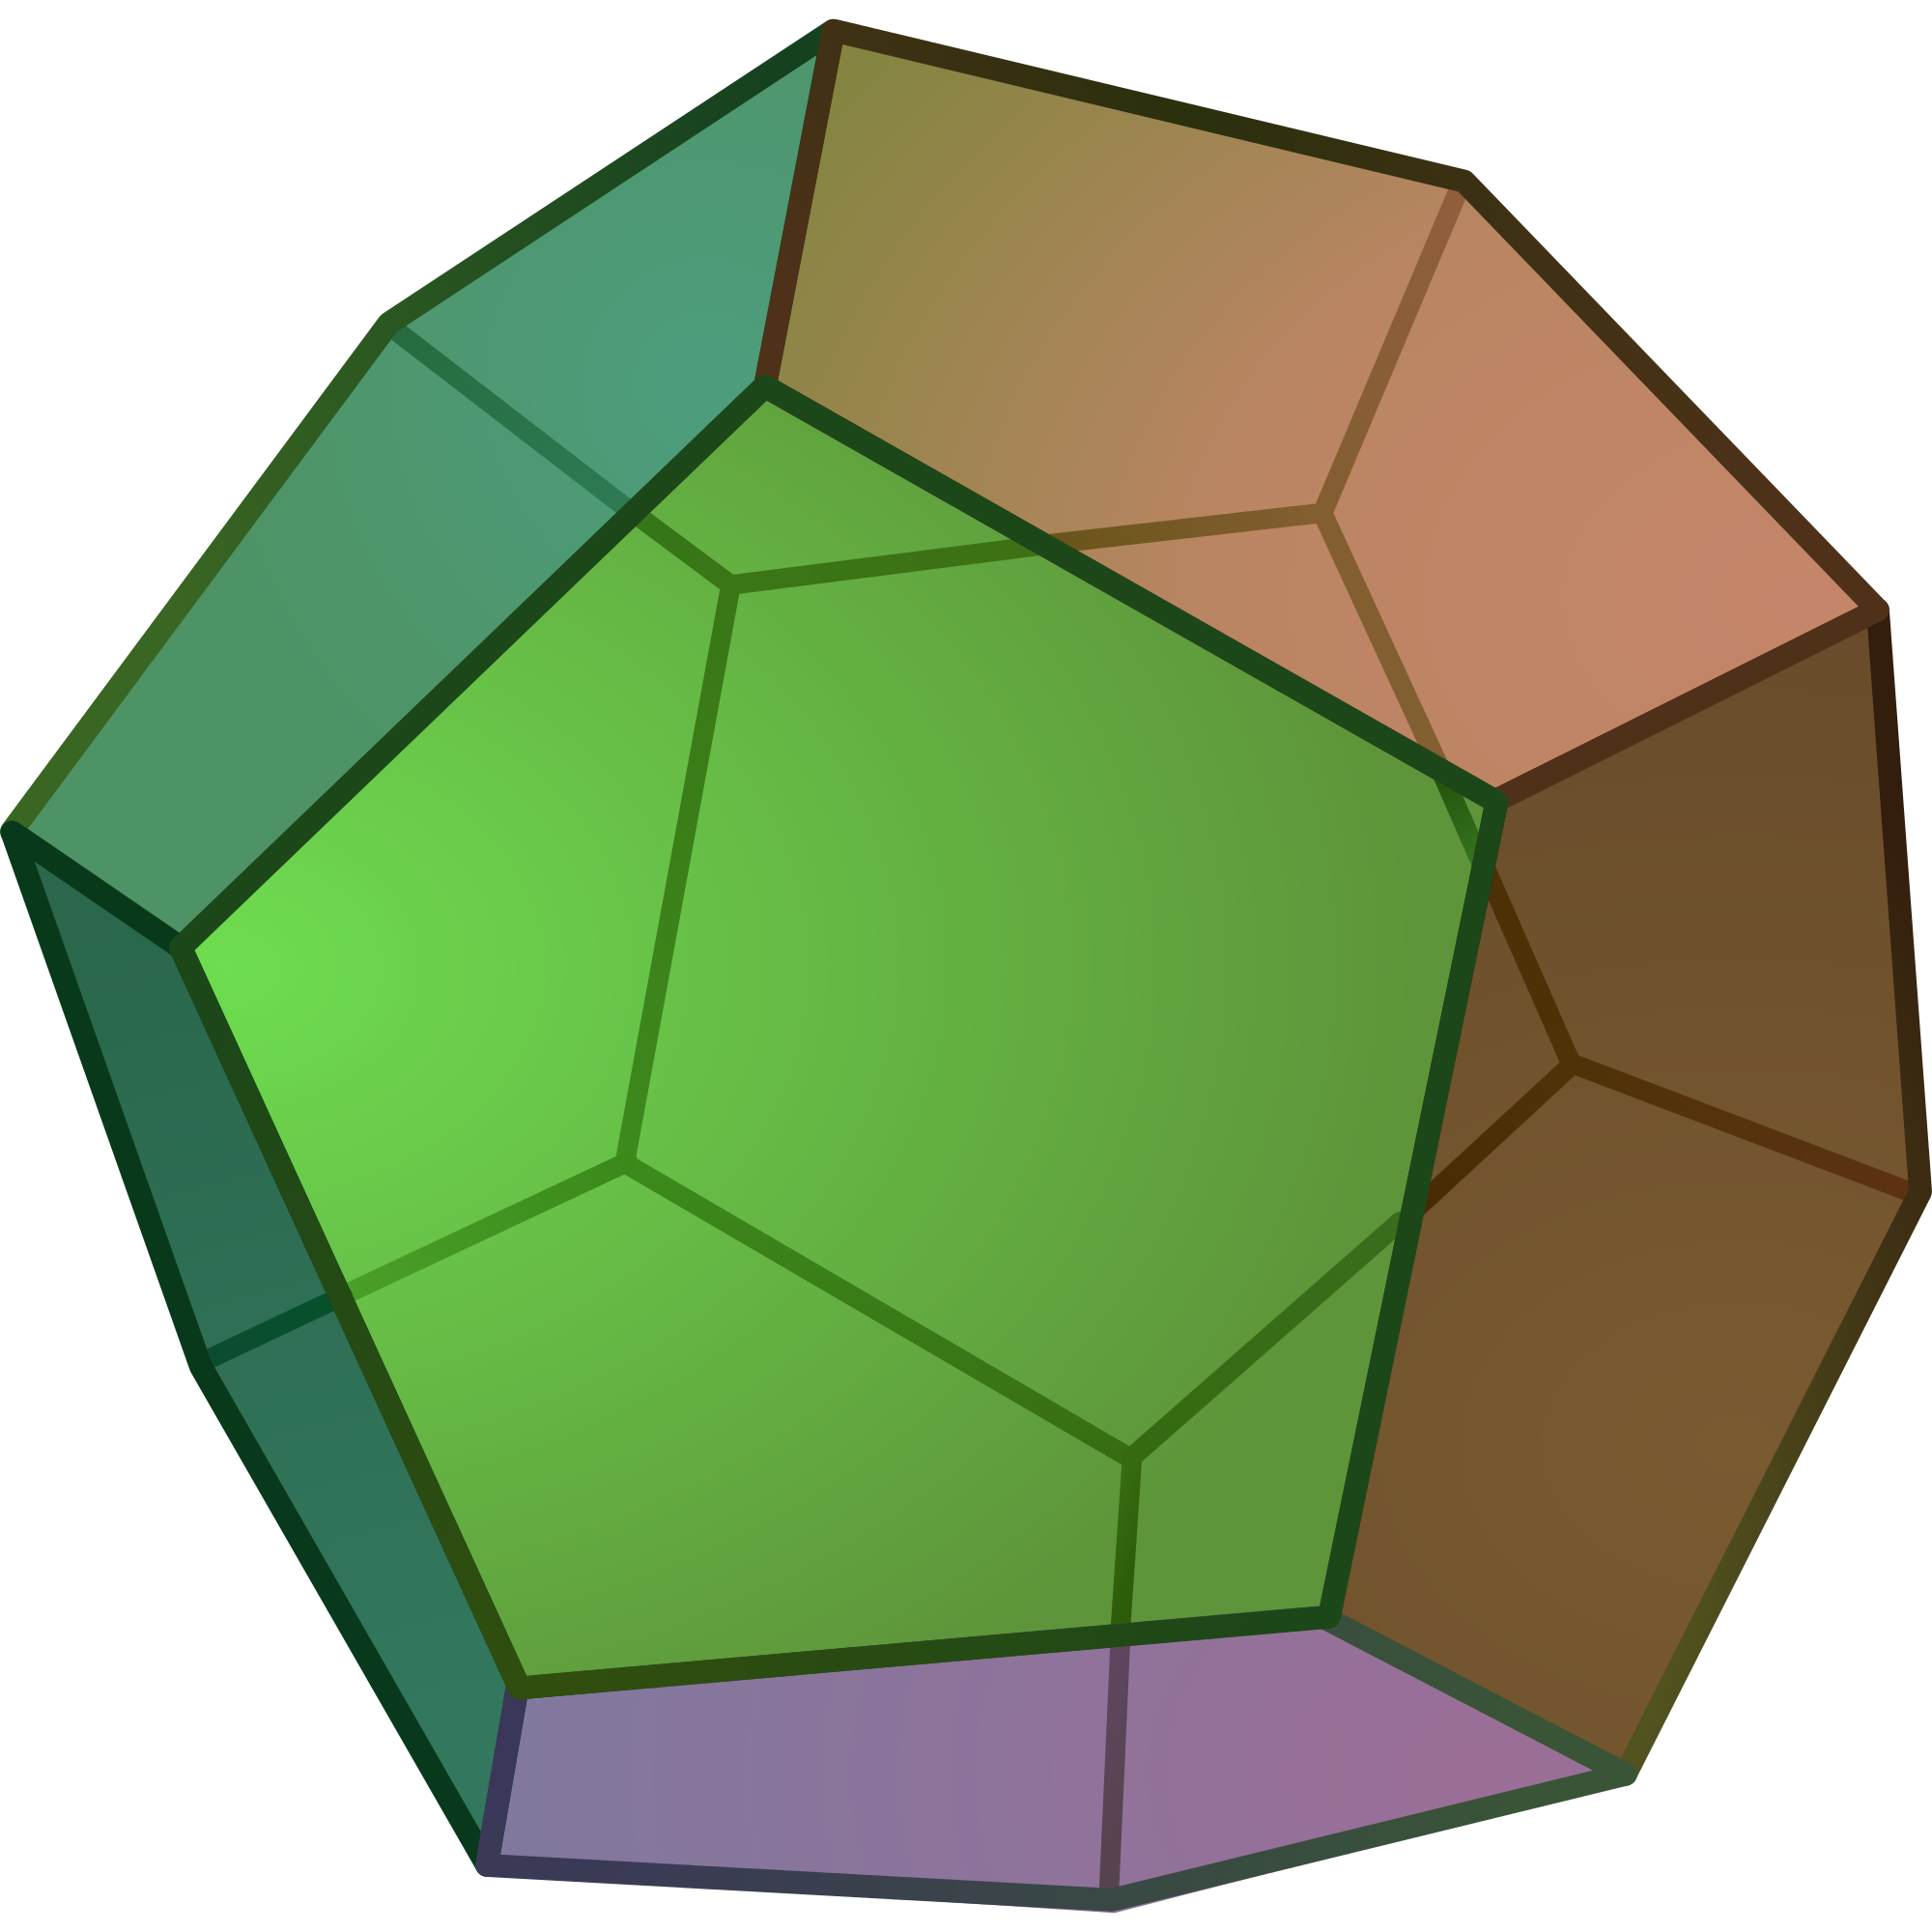
\includegraphics{dodecahedron.png}
        \end{figure}
      }

      Dodecahedron
     \end{column}
\end{columns}
\btVFill
\textit{\scriptsize Image credit: Wikipedia users DTR, Stannered}
%<1->
\end{frame}
% -----------------------------------------------------------------------------
\begin{frame}{Archimedean Solids}
\begin{itemize}
  \item Composed of more than one type of regular polygon
  \item Identical vertices
  \item 13 Archimedean Solids
\end{itemize}
\vspace{0.1 in}
\begin{columns}
    \begin{column}{0.32\textwidth}
      \centering
      %Octahedron
      
      \scalebox{0.06}{
        \begin{figure}
          \centering
          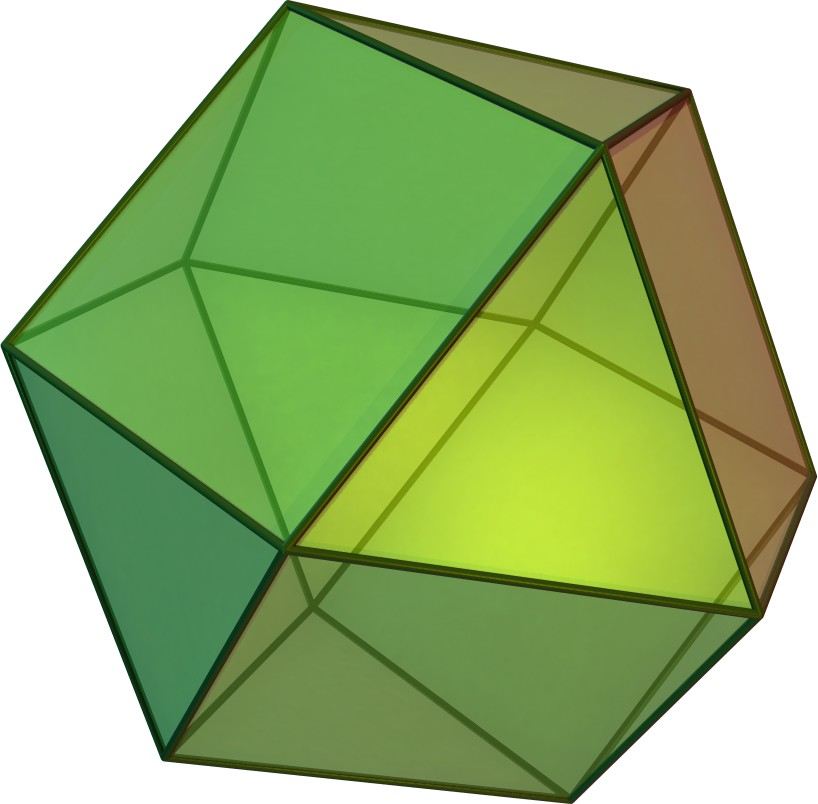
\includegraphics{cuboctahedron.jpg}
        \end{figure}
      }

      Cuboctahedron
     \end{column}
    \begin{column}{0.32\textwidth}
      \centering
      %Cube

      \scalebox{0.06}{
        \begin{figure}
          \centering
          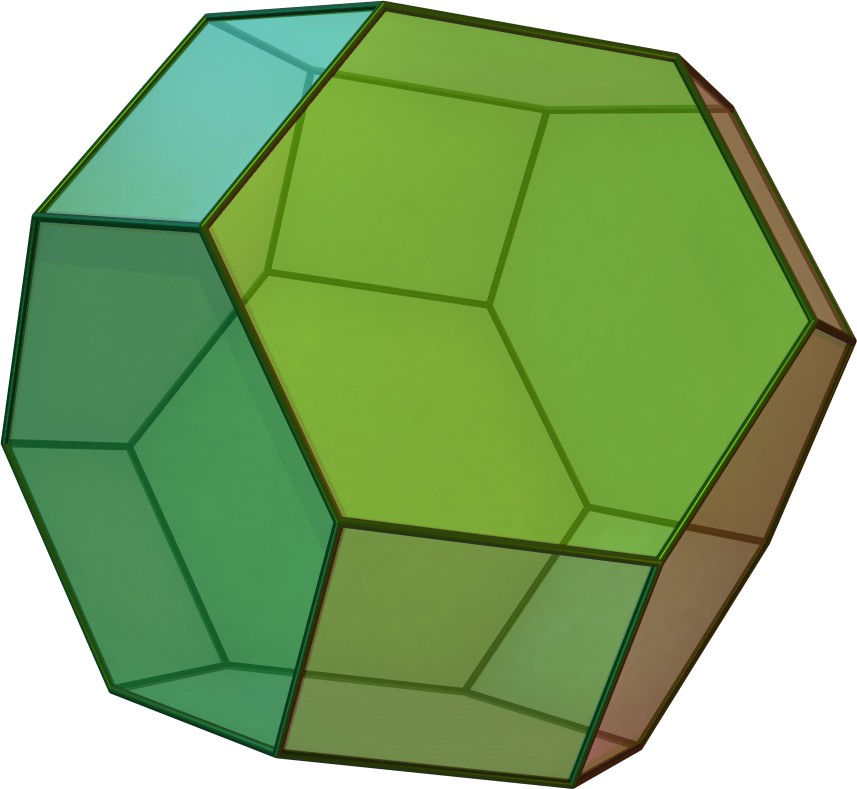
\includegraphics{truncated_octahedron.jpg}
        \end{figure}
      }

      Truncated Octahedron
     \end{column}
    \begin{column}{0.32\textwidth}
      \centering
      
      \scalebox{0.06}{
        \begin{figure}
          \centering
          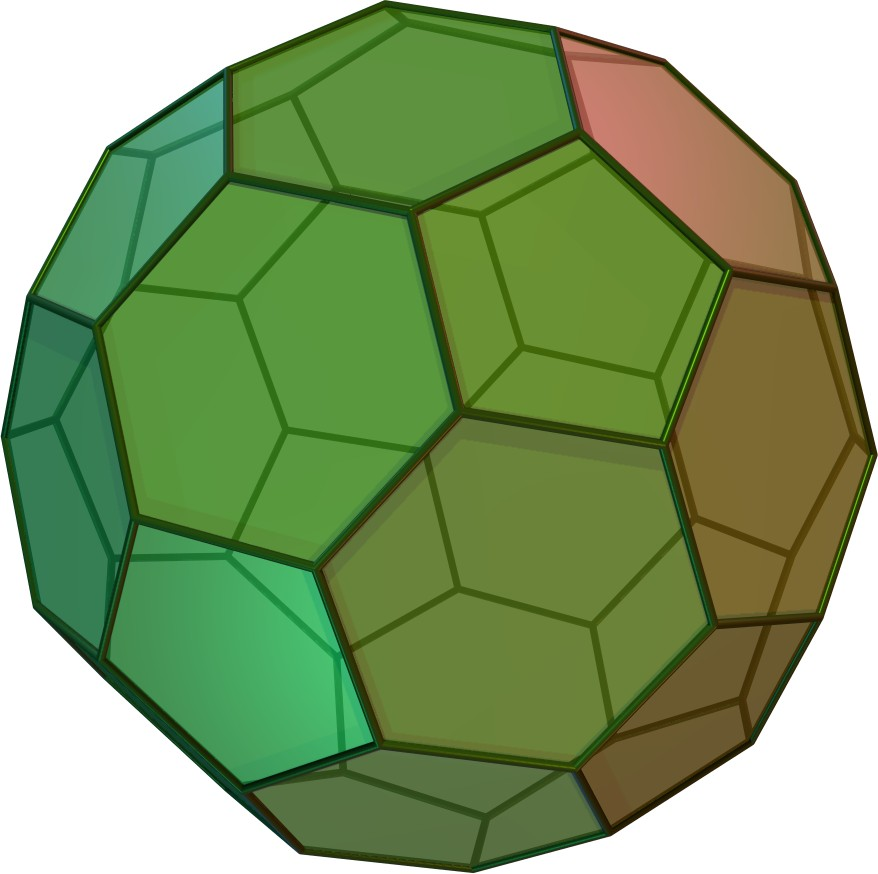
\includegraphics{truncated_icosahedron.jpg}
        \end{figure}
      }

      Truncated Icosahedron
     \end{column}
\end{columns}
\btVFill
\textit{\scriptsize Image credit: Wikipedia user Cyp}
\end{frame}
% -----------------------------------------------------------------------------
\begin{frame}{Catalan Solids}
\begin{itemize}
  \item Composed of a single type of non-regular polygon
  \item Dual to Archimedean solids
  \item 13 Catalan Solids
\end{itemize}
\vspace{0.1 in}
\begin{columns}
    \begin{column}{0.32\textwidth}
      \centering
      %Cube

      \scalebox{0.06}{
        \begin{figure}
          \centering
          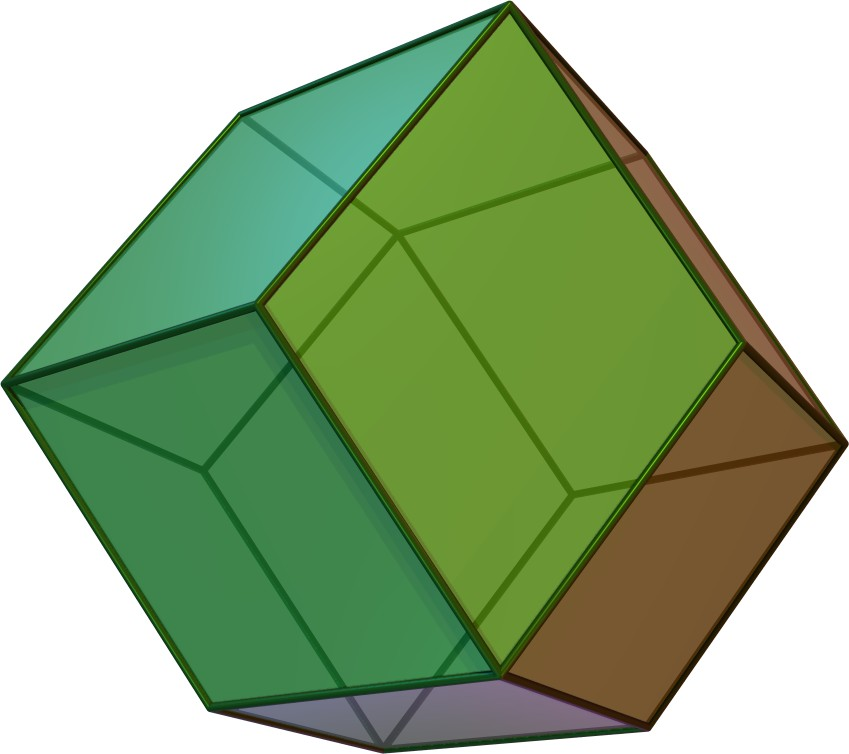
\includegraphics{rhombicdodecahedron.jpg}
        \end{figure}
      }

      Rhombic Dodecahedron
     \end{column}
    \begin{column}{0.32\textwidth}
      \centering
      %Octahedron
      
      \scalebox{0.06}{
        \begin{figure}
          \centering
          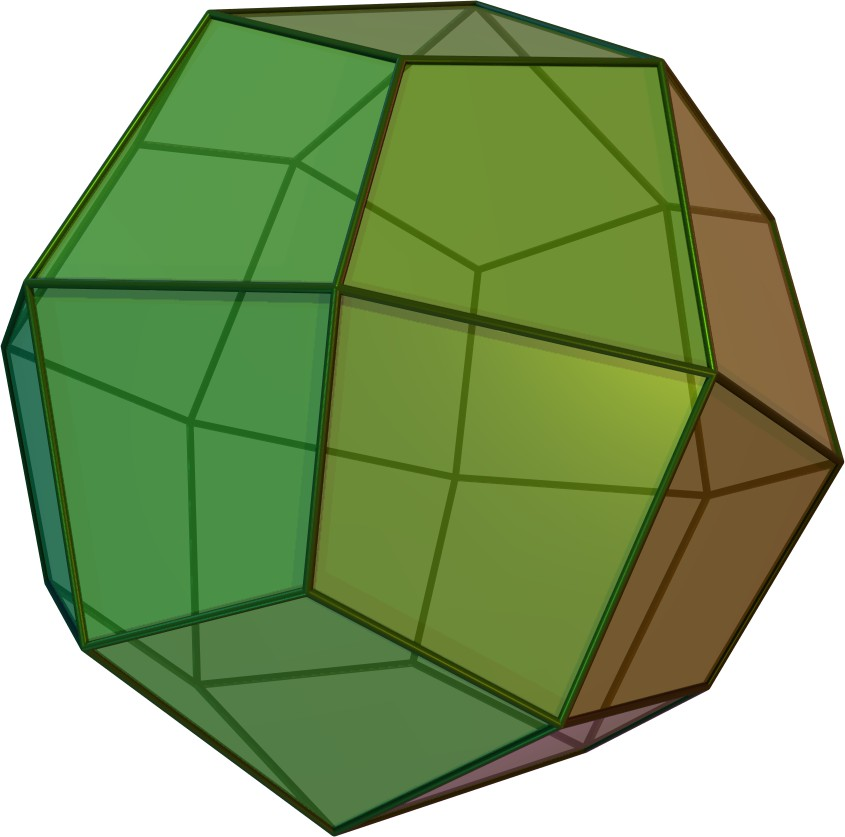
\includegraphics{deltoidal_icositetrahedron.jpg}
        \end{figure}
      }

      Deltoidal Icositetrahedron
     \end{column}
    \begin{column}{0.32\textwidth}
      \centering
      
      \scalebox{0.06}{
        \begin{figure}
          \centering
          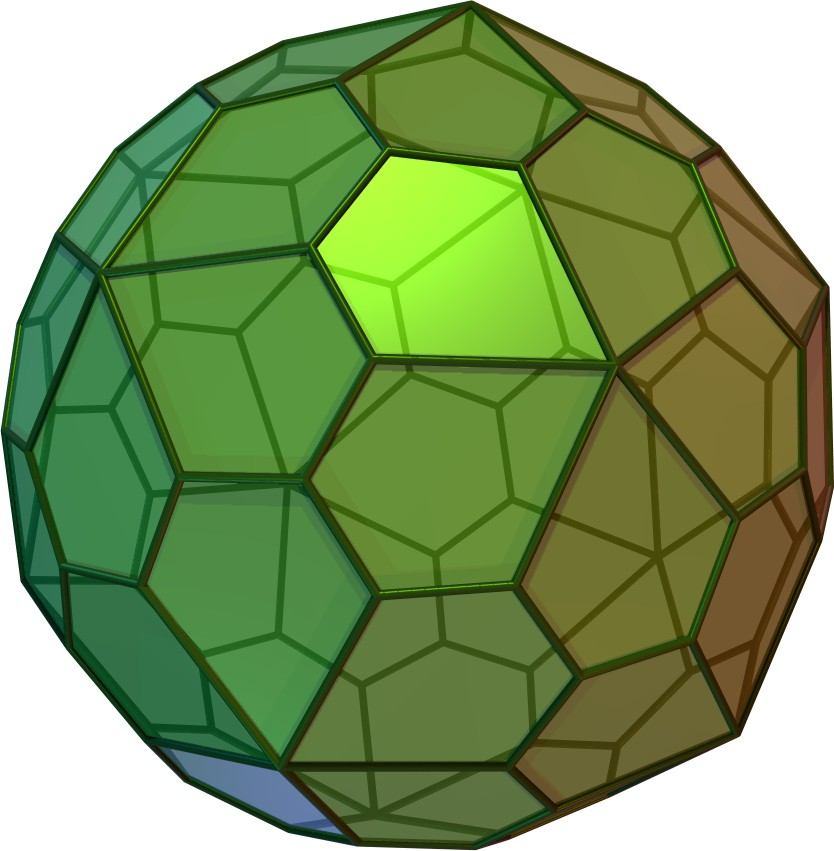
\includegraphics{pentagonal_hexecontahedron.jpg}
        \end{figure}
      }

      Pentagonal Hexecontahedron
     \end{column}
\end{columns}
\btVFill
\textit{\scriptsize Image credit: Wikipedia users Cyberpunk and Maxim Razin}
\end{frame}
% -----------------------------------------------------------------------------
%\subsection{Scientific Motivation}
\begin{frame}{Viral Capsids}
%\begin{columns}
%    \begin{column}{0.48\textwidth}
%
%    \end{column}
%    \begin{column}{0.48\textwidth}
%    \scalebox{0.19}{
%      \begin{figure}
%        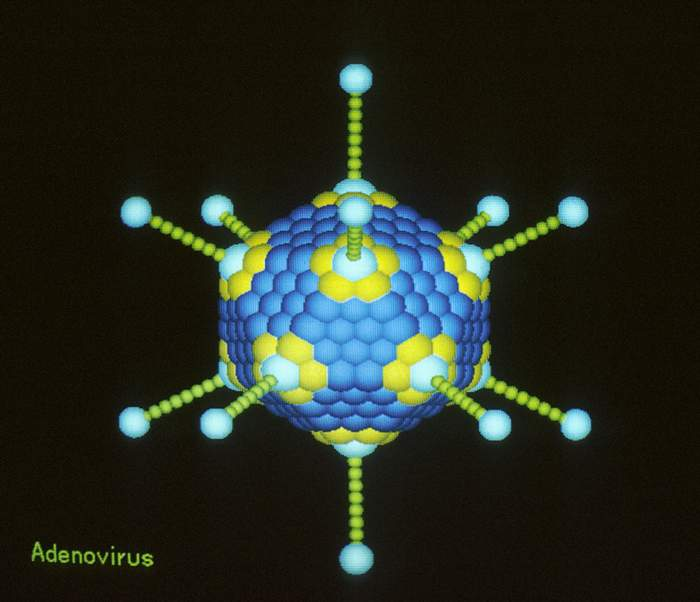
\includegraphics{Adenovirus.jpg}
%        %\hspace*{15pt}\hbox{\scriptsize Credit:\thinspace{\small\itshape National Cancer Institute}}
%        %\caption{Credit: National Cancer Institute}
%       \end{figure}
%     }
%    \end{column}
%\end{columns}
  \centering
    \scalebox{0.25}{
      \begin{figure}
        \centering
        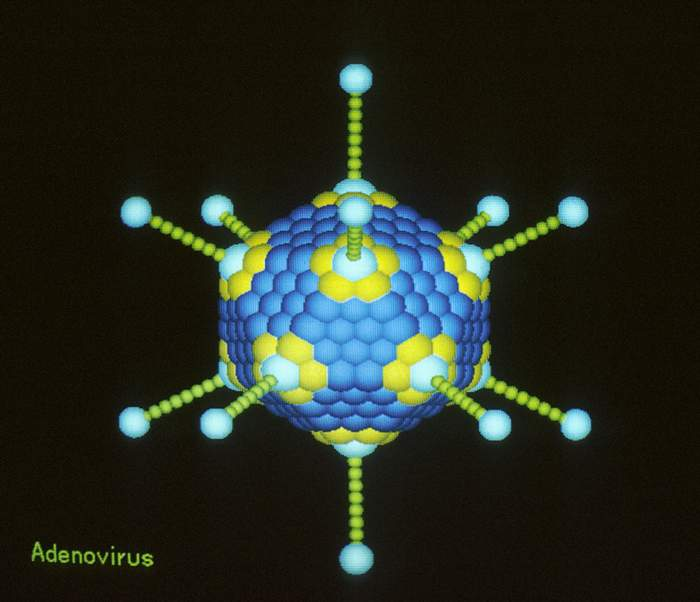
\includegraphics{Adenovirus.jpg}
       \end{figure}
     }
       %\caption{Credit: National Cancer Institute}
\btVFill
\textit{\scriptsize Image credit: National Cancer Institute} 
\end{frame}
% -----------------------------------------------------------------------------
\begin{frame}{Molecular Cages}
%\begin{columns}
%    \begin{column}{0.48\textwidth}
%
%    \end{column}
%    \begin{column}{0.48\textwidth}
%    \scalebox{0.1}{
%      \begin{figure}
%        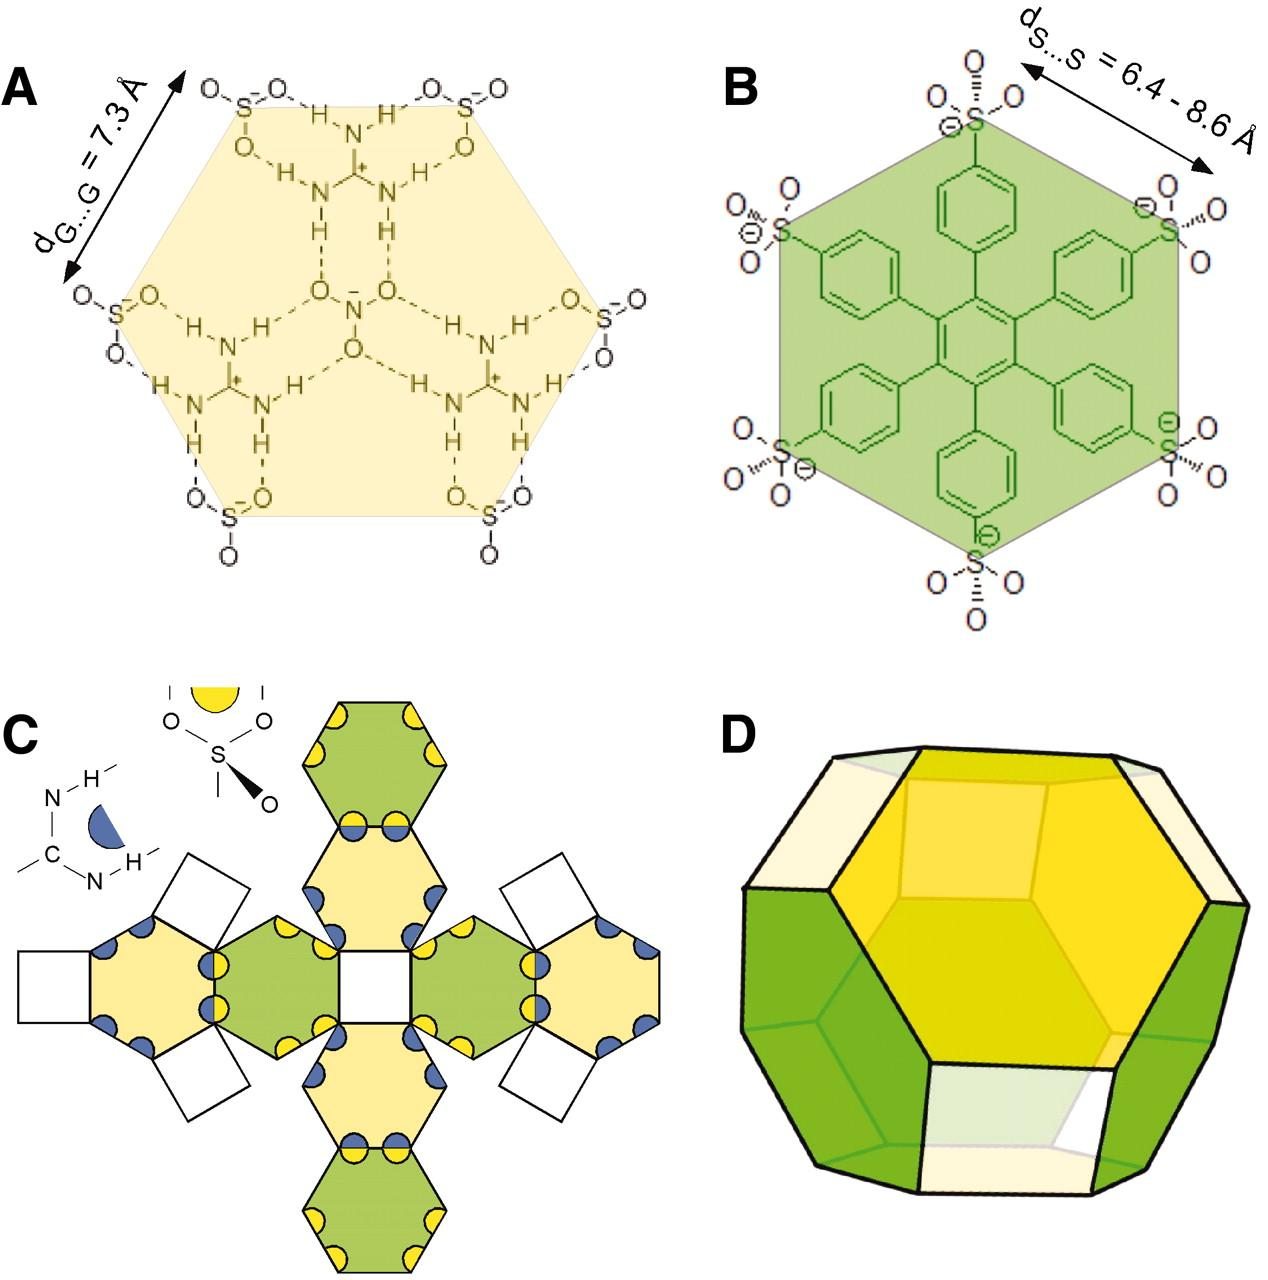
\includegraphics{ward_cage.png}
%        %\hspace*{15pt}\hbox{\scriptsize Credit:\thinspace{\small\itshape National Cancer Institute}}
%        %\caption{Credit: National Cancer Institute}
%       \end{figure}
%      }
%    \end{column}
%\end{columns}
  \centering
    \scalebox{0.12}{
      \begin{figure}
        \centering
        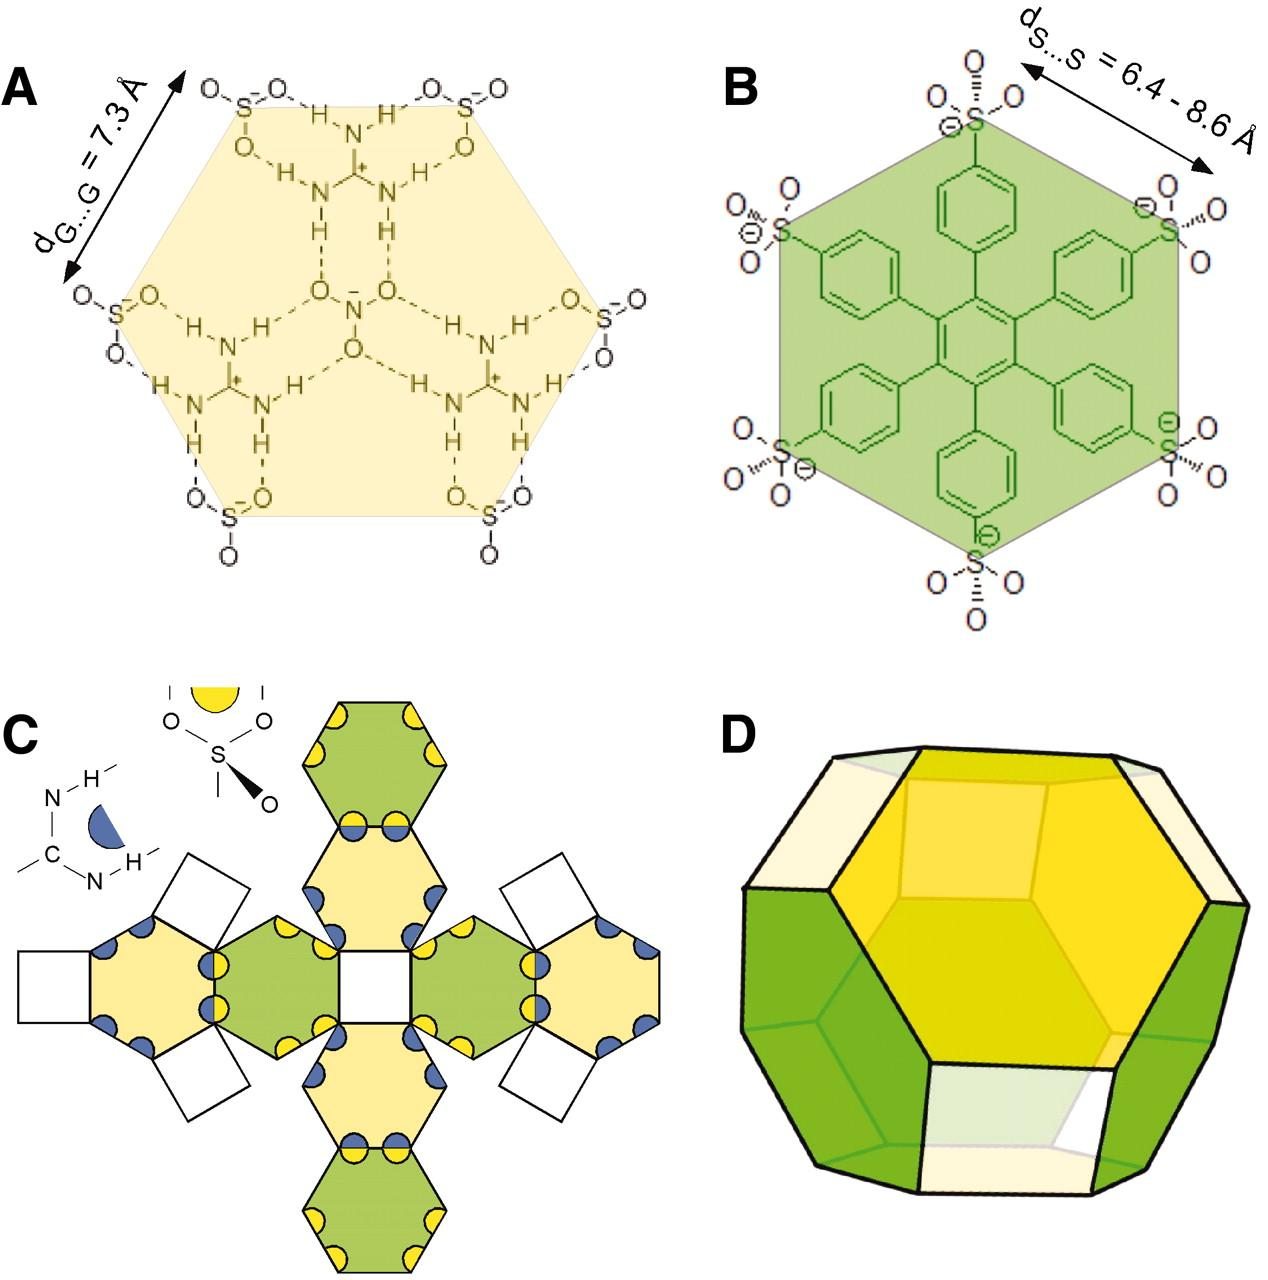
\includegraphics{ward_cage.png}
       \end{figure}
      }
\btVFill
\textit{\scriptsize Image credit: Ward Research Group, NYU} 
\end{frame}
% -----------------------------------------------------------------------------
\begin{frame}{Self-Folding Polyhedra}
  \centering
    \scalebox{0.12}{
      \begin{figure}
        \centering
        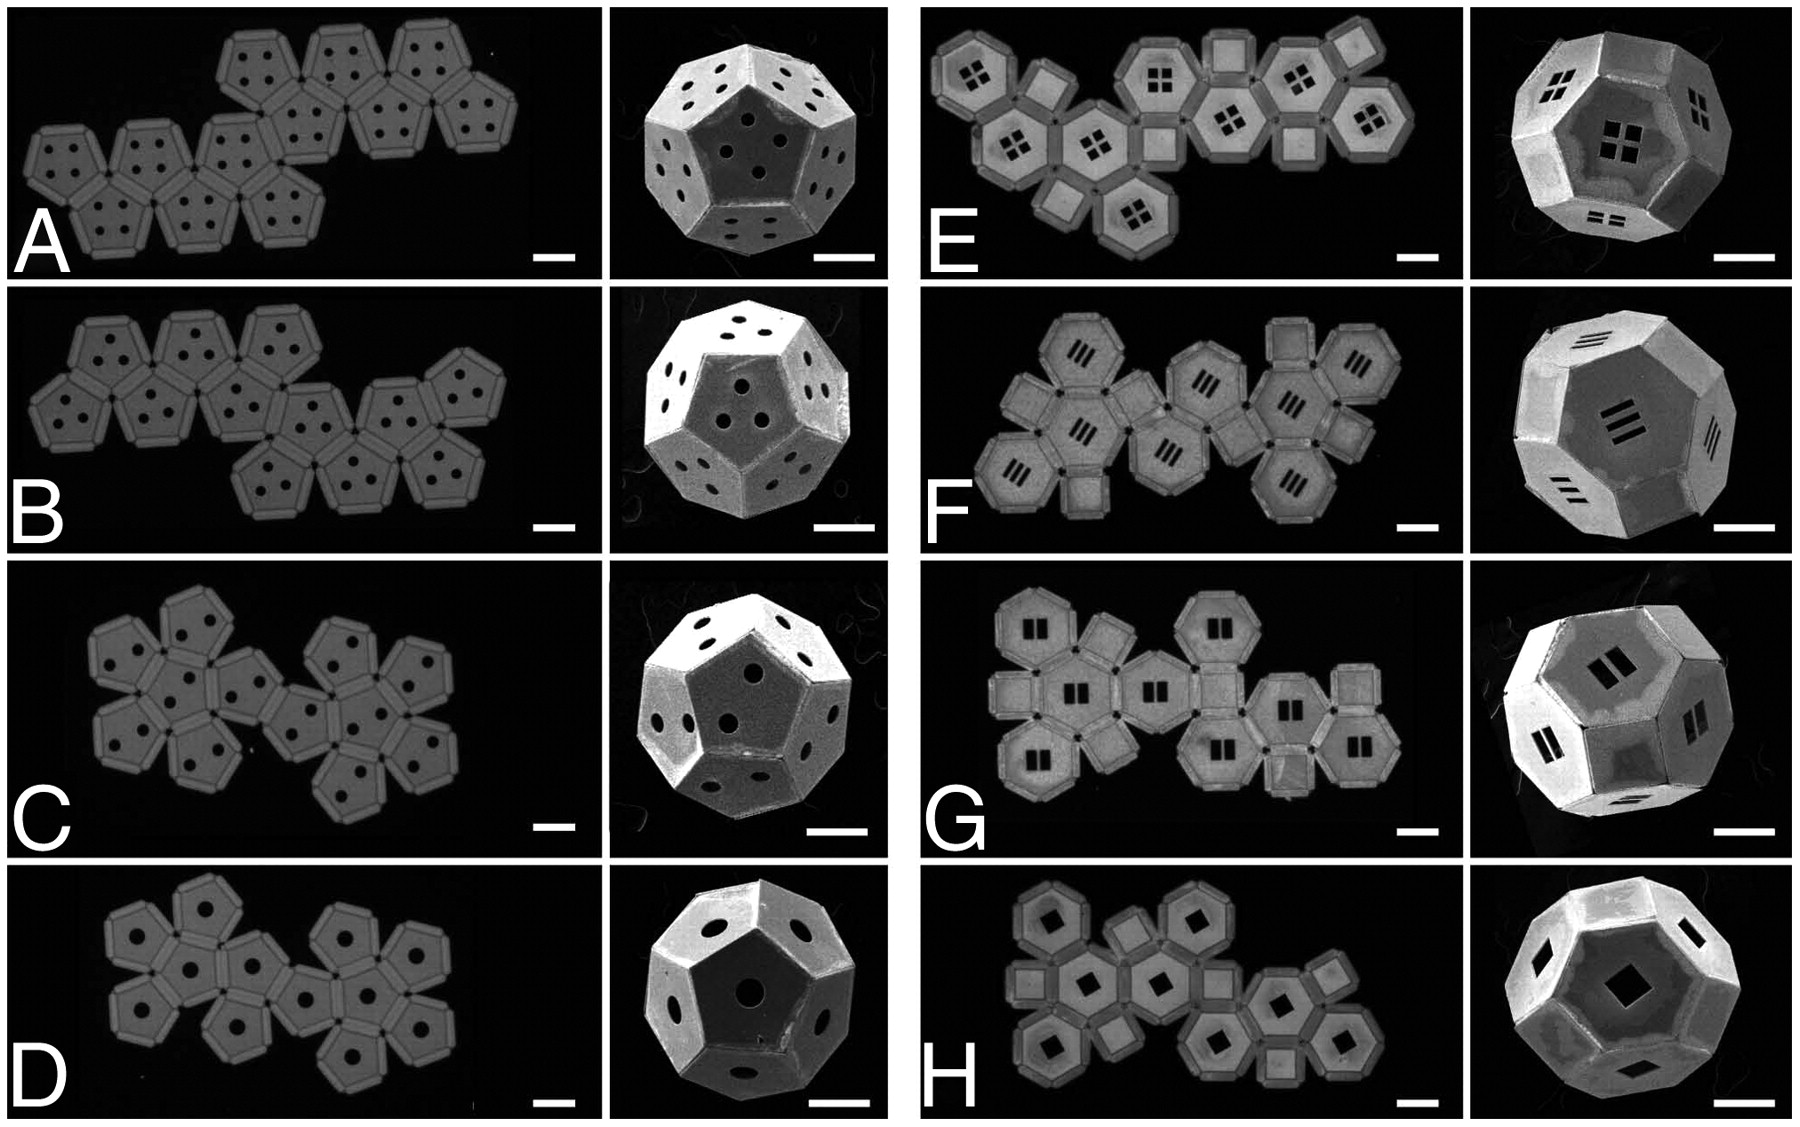
\includegraphics{gracias.png}
       \end{figure}
      }
\btVFill
\textit{\scriptsize Image credit: Gracias Group, Johns Hopkins} 
\end{frame}
% -----------------------------------------------------------------------------
\begin{frame}{Other Applications}
\begin{columns}
    \begin{column}{0.48\textwidth}
%        \includegraphics[width=<X>\textwidth]{}
\scalebox{0.19}{
        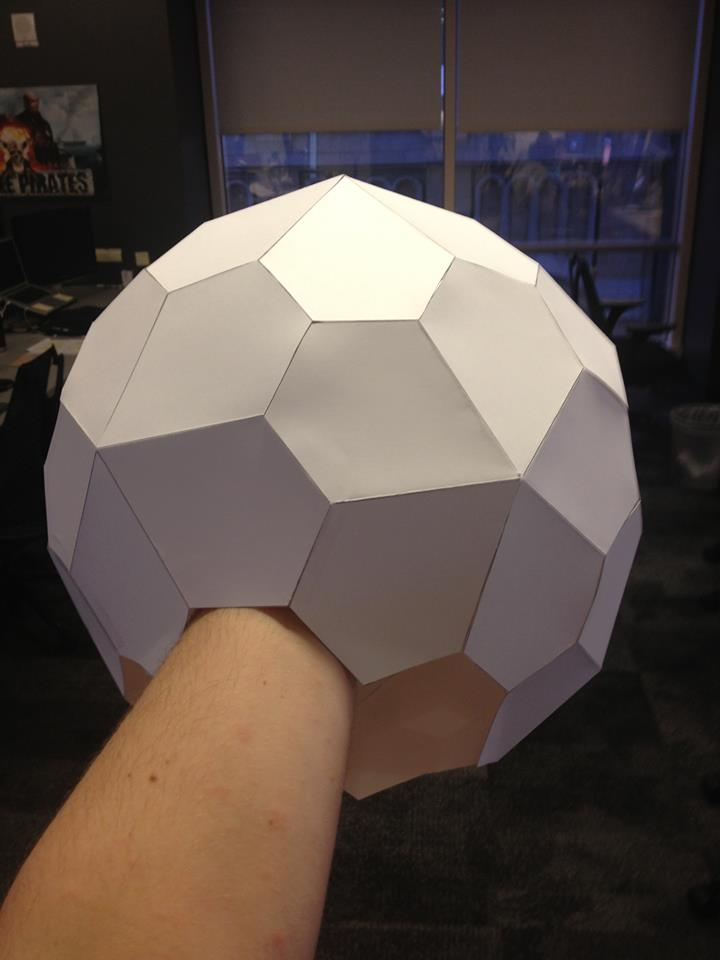
\includegraphics{jeremy_polyhedra.jpg}
}
    \end{column}
    \begin{column}{0.48\textwidth}
\scalebox{0.19}{
        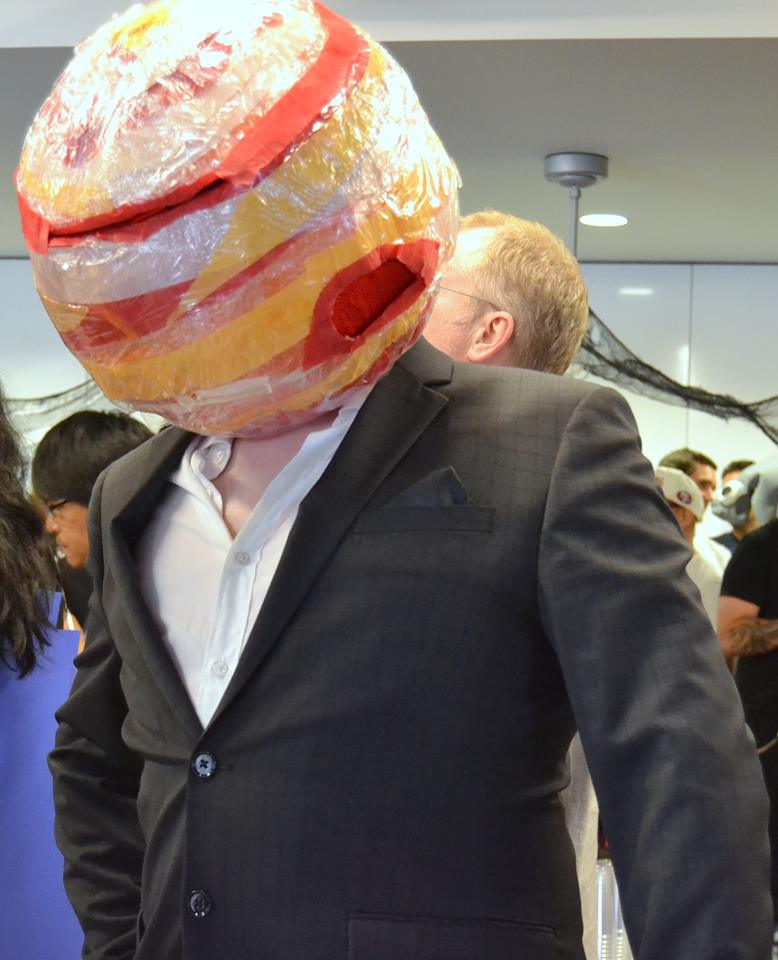
\includegraphics{mr_jupiter.jpg}
}
    \end{column}
\end{columns}
\end{frame}
% -----------------------------------------------------------------------------
% -----------------------------------------------------------------------------
\section{The Building Game}
%% -----------------------------------------------------------------------------
%\begin{frame}{Sequential Attachment}
%MOVIE??
%\end{frame}
% -----------------------------------------------------------------------------
%\subsection{Definitions}
\begin{frame}{The Building Game}
%\begin{columns}
%    \begin{column}{0.48\textwidth}
%
%    \end{column}
%    \begin{column}{0.48\textwidth}
%    \scalebox{0.25}{
%      \begin{figure}
%        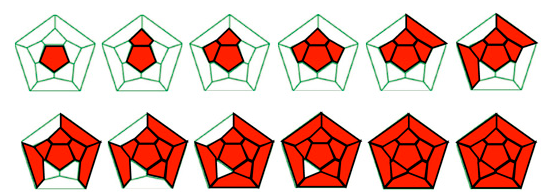
\includegraphics{bg.png}
%       \end{figure}
%      }
%    \end{column}
%\end{columns}
  \centering
    \scalebox{0.04}{
      \begin{figure}
        \centering
        \includegraphics{octa_path.pdf}
        %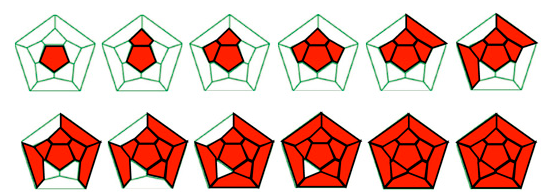
\includegraphics{bg.png}
       \end{figure}
      }
\begin{itemize}
  \item Begin with a single face.
  \item At each step, add a face adjacent to an already added face.
  \item End when all faces have been added.
\end{itemize}

%\btVFill
%\textit{\scriptsize Image credit: Govind Menon, Brown} 

\end{frame}
% -----------------------------------------------------------------------------
\begin{frame}{States and Intermediates}
\begin{definition}
  A Building Game \textbf{state} $x$ is a non-empty subset of the faces $F$ of a polyhedron such that the subset is connected along edges. 
\end{definition} 
\begin{definition}
A Building Game \textbf{intermediate} $[x]$ is an equivalence class on states given by the equivalence relation: $x \sim \hat{x}$ if $x$ can be rotated to get $\hat{x}$.
\end{definition}

\end{frame}
% -----------------------------------------------------------------------------
\begin{frame}{Connections and Pathways}
\begin{definition}
A \textbf{connection} exists between two intermediates if one can be formed by adding a face to the other.
\end{definition}
\begin{definition}
A building game \textbf{pathway} is an increasing sequence of intermediates that begins with a single face, proceeds with consecutive intermediates being connected, and finishes with the completed polyhedron.
\end{definition}

\end{frame}
% -----------------------------------------------------------------------------
\begin{frame}{Degeneracies}
\begin{definition}
The \textbf{degeneracy number} $S_{jk}$ for a connection is the number of different faces that can be added to (or removed from) one intermediate $[x^j]$ to form the other $[x^k]$.    
\end{definition}
The degeneracy number is not symmetric in general: $S_{jk} \neq S_{kj}$.

\centering
    \scalebox{0.24}{
        \centering
        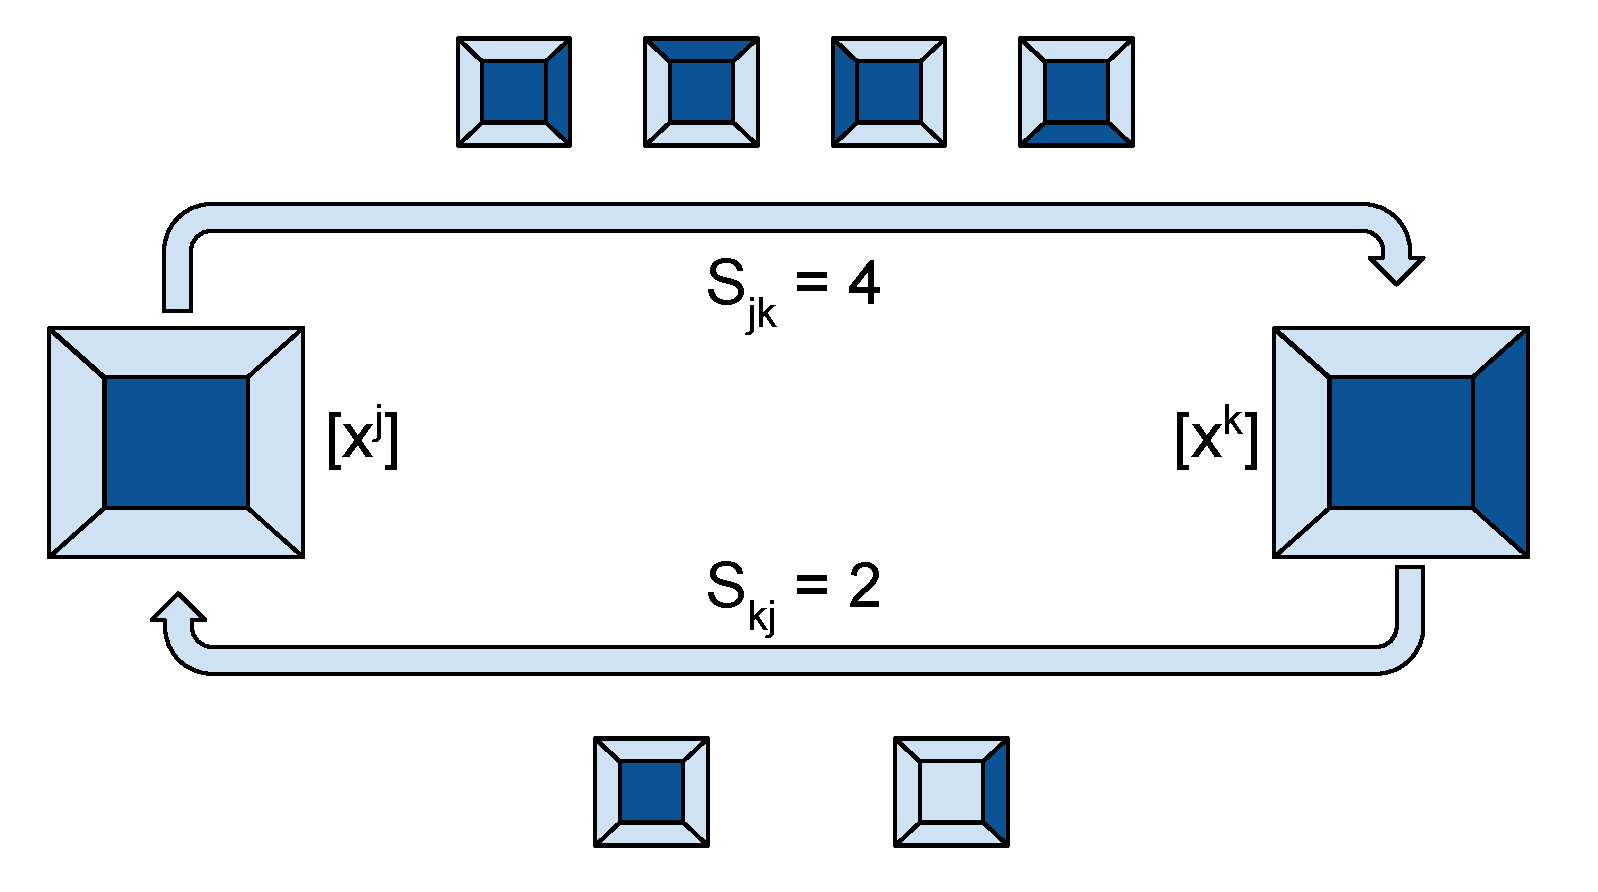
\includegraphics{degeneracies.pdf}
      }
\end{frame}
% -----------------------------------------------------------------------------
\begin{frame}{Combinatorial Configuration Space: Cube}
    \scalebox{0.4}{
      \begin{figure}
        \centering
        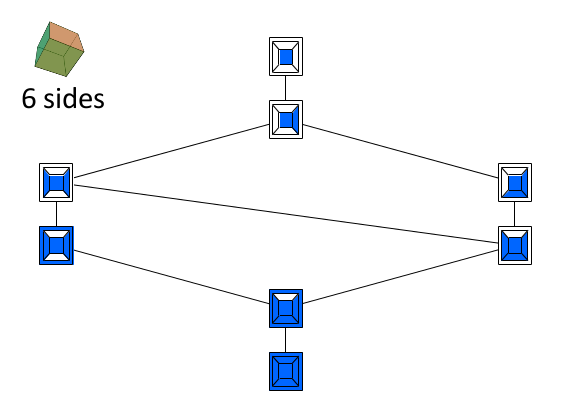
\includegraphics{cube_bg.png}
       \end{figure}
      }
\end{frame}
% -----------------------------------------------------------------------------
\begin{frame}{Combinatorial Configuration Space: Dodecahedron}
    \scalebox{0.4}{
      \begin{figure}
        \centering
        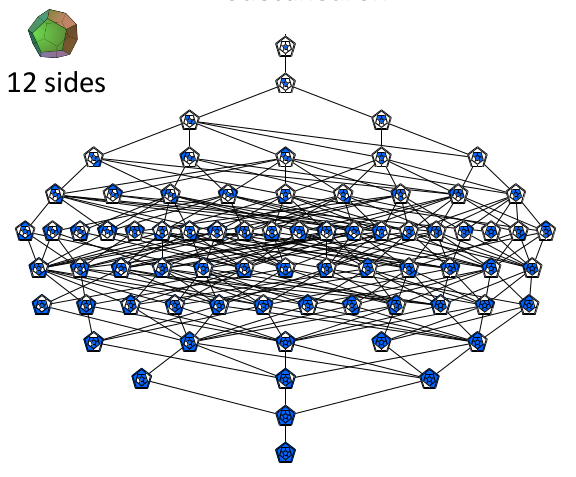
\includegraphics{dodecahedronSS.png}
       \end{figure}
      }
\end{frame}
% -----------------------------------------------------------------------------
\begin{frame}{Configuration Space Statistics}
\begin{figure}[ht]
\scalebox{0.5}{
%{\footnotesize
\centering
%\textbf{Building Game Enumerative Results for the Platonic Solids}
\begin{tabular}{ l | c | r | r | r}
Polyhedron Name & $|F|$ & Intermediates & Connections & Pathways \\
  \hline    
Tetrahedron                     & 4        & 4     	& 3             & 1\\
Cube                            & 6        & 8     	& 9    		& 3\\
Octahedron                      & 8        & 14    	& 21    	& 14\\
Dodecahedron                    & 12       & 73    	& 263   	& 17,696 \\
Icosahedron                     & 20       & 2,649 	& 17,241        & 57,396,146,640\\ \hline
Truncated Tetrahedron           & 8     & 28    	& 63            & 402\\
Cuboctahedron                   & 14  	& 340   	& 1,634         & 10,170,968\\
Truncated Cube                  & 14  	& 499   	& 2,729         & 101,443,338 \\
Truncated Octahedron            & 14  	& 555           & 3,069         & 68,106,377\\
Rhombicuboctahedron             & 26  	& 638,850       & 6,459,801     & 164,068,345,221,515,292,308\\
Truncated Cuboctahedron         & 26  	& 1,525,658     & 17,672,374    & 13,837,219,462,483,379,105,902\\ \hline  
Triakis Tetrahedron             & 12  	& 98            & 318           & 38,938\\
Rhombic Dodecahedron            & 12  	& 127           & 493           & 76,936\\
Triakis Octahedron              & 24  	& 12,748        & 81,296        & 169,402,670,046,670\\
Tetrakis Hexahedron             & 24  	& 50,767        & 394,377       & 4,253,948,297,210,346\\
Deltoidal Icositetrahedron      & 24  	& 209,675       & 1,989,548     & 418,663,242,727,526,726 \\
Pentagonal Icositetrahedron     & 24  	& 345,938       & 3,544,987     & 2,828,128,000,716,774,492\\
Rhombic Triacontahedron         & 30  	& 2,423,212     & 26,823,095    & 161,598,744,916,797,017,978,128\\
\end{tabular}
}
%\caption{Building game combinatorial configuration space enumerative results for the Platonic, Archimedean, and Catalan solids.}
\label{tab:bgEnum}
\end{figure}

\end{frame}
% -----------------------------------------------------------------------------

\begin{frame}{Computation}
\begin{itemize}
\item Given all intermediates with $k$ faces, compute the ones with $k+1$ faces.
\item Brute force approach necessary.  
\item Comparing two states for equivalence uses hash function. 
\item Limited by combinatorial explosion of configuration space size.
\end{itemize}
\end{frame}

% -----------------------------------------------------------------------------
% -----------------------------------------------------------------------------
\section{Stochastic Modeling}
% -----------------------------------------------------------------------------
%\subsection{Stochastic Modeling} 
\begin{frame}{Energy Landscape Model}
  \centering
    \scalebox{0.4}{
      \begin{figure}
        \centering
        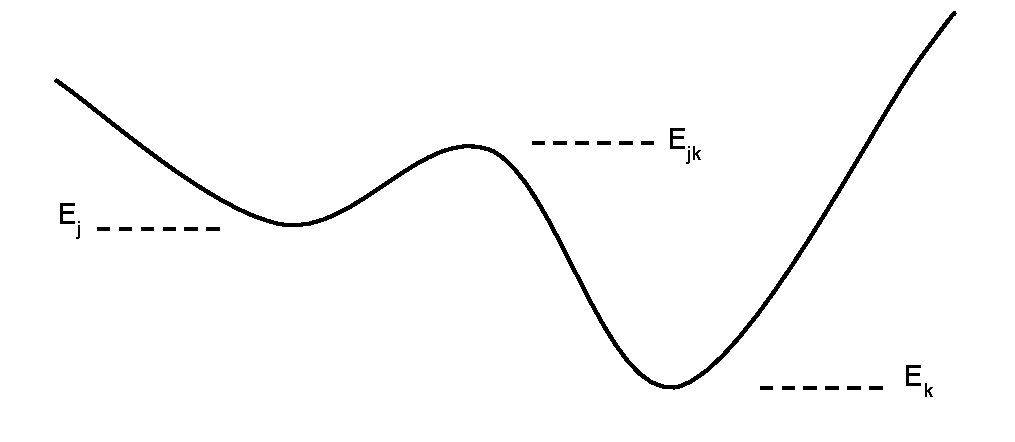
\includegraphics{energy_landscape.pdf}
       \end{figure}
      }
%$$\log\left(P([x^j] \to [x^k]) \right) \propto -\beta(E_{jk} - E_j)$$
\begin{itemize}
\item $\log\left(Q_{jk} \right) \propto -\beta(E_{jk} - E_j)$
\item Choose $E_j = -\#\left(\text{closed edges}\right)$ to model satisfied bonds.
\end{itemize} 
\end{frame}
% -----------------------------------------------------------------------------
\begin{frame}{Markov Processes}
\begin{itemize}
\item $X_t$ a continuous time Markov process on the configuration space graph.
\item Transition rates given by matrix $Q$
\end{itemize}
\begin{align}
  \label{eq:Qdef}
  Q_{jk} &=
  \begin{cases}
   S_{jk}e^{-\beta\left(E_{jk} - E_{j}\right)} & \text{if } [x^j] \leftrightarrow [x^k]  \\
   -z_j       & \text{if } j = k \\
   0 & \text{else}
  \end{cases} \\
z_j &= \sum_{\ell: \ell \neq j} S_{j\ell}e^{-\beta\left(E_{j\ell} - E_j\right)}
\end{align}
\end{frame}
% -----------------------------------------------------------------------------


\begin{frame}{Stationary Distribution}
\begin{theorem}
The Markov process $X_t$ with rate matrix $Q$ has stationary distribution $\pi$.
$$\pi_j &= \frac{1}{Zr_j}e^{-\beta E_j}$$
\end{theorem}
\begin{lemma}
There is the following relation between degeneracy numbers and symmetry numbers.
$$ r_jS_{kj} = r_{k}S_{jk}$$
\end{lemma}
\end{frame}
% -----------------------------------------------------------------------------
\begin{frame}{Stationary Distribution II}
\begin{proof}
Detailed Balance!
\begin{align}
\pi_jQ_{jk} &= \left(\frac{1}{Zr_j}e^{-\beta E_j}\right)\left(S_{jk}e^{-\beta\left(E_{jk} - E_j\right)}\right) \\
&= \left(\frac{1}{Z}e^{-\beta E_{jk}}\right)\left(\frac{S_{jk}}{r_j}\right) \\
&= \left(\frac{1}{Z}e^{-\beta E_{kj}}\right)\left(\frac{S_{kj}}{r_k}\right) \\
&= \pi_kQ_{kj}
\end{align}
\end{proof}
\end{frame}
% -----------------------------------------------------------------------------
\begin{frame}{Formation Times}
Under our Markov process model, how long does it take to form the polyhedron on average?

$$\tau_{j} &\doteq \inf\left\{t \geq 0 : X_t = [F], X_0 = [x^j]\right\}$$

$$E\left[\tau^{[F]}\right] &= \left[\left(\diag\left(\mathbbm{1}_{[F]}\right) - \diag\left(\mathbbm{1}_{[F]^c}\right)Q\right)\right]^{-1} \mathbbm{1}_{[F]^c}$$
  \centering
    \scalebox{0.4}{
      \begin{figure}
        \centering
        NEWFIG
        %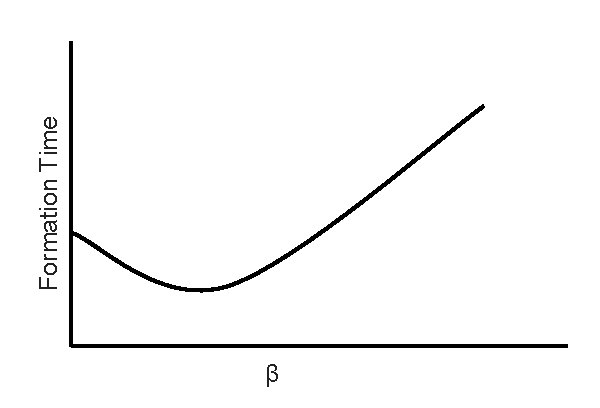
\includegraphics{formation_time.pdf}
       \end{figure}
      }
\end{frame}

% -----------------------------------------------------------------------------
% -----------------------------------------------------------------------------
\section{Geometric Configuration Space}
% -----------------------------------------------------------------------------
\begin{frame}{Polygonal Linkage}
MOVIE
\end{frame}
% -----------------------------------------------------------------------------
\begin{frame}{Constraint Model}
\begin{itemize}
\item Use constraint equations to enforce rigidity of polygonal faces and hinged motion along connected edges.
\item $z = [v_1^T, v_2^T, \dots, v_{n/3}^T]^T \in \mathbbm{R}^n$
\item Constraint function $c: \mathbbm{R}^n \to \mathbbm{R}^m$
\item Length constraint $c_j(z) = |v_{j_a} - v_{j_b}|^2 - 1$
%\item Solution set $\mathcal{M} \doteq \{z \in \mathbbm{R}^n: c(z) = 0\}$ an algebraic variety
\end{itemize}
\begin{definition}
The \textbf{geometric configuration space} is the algebraic variety $\mathcal{M} \doteq \{z \in \mathbbm{R}^n: c(z) = 0\}$. 
\end{definition}

\end{frame}
%% -----------------------------------------------------------------------------
%\begin{frame}{Geometric Configuration Space}
%Definition
%\end{frame}
% -----------------------------------------------------------------------------
\begin{frame}{Degrees of Freedom}
\begin{definition}
The number of \textbf{degrees of freedom} a Building Game intermediate at configuration $z$ is the dimension of the geometric configuration space $\mathcal{M}$ at $z$. 
\end{definition}
\begin{itemize}
\item Six \textit{trivial degrees of freedom}: rigid body translations and rotations. 
\item Remaining are \textit{internal degrees of freedom}
\end{itemize}
\end{frame}
%% -----------------------------------------------------------------------------
\begin{frame}{Degrees of Freedom: Dodecahedron}
  \centering
\scalebox{0.6}{
        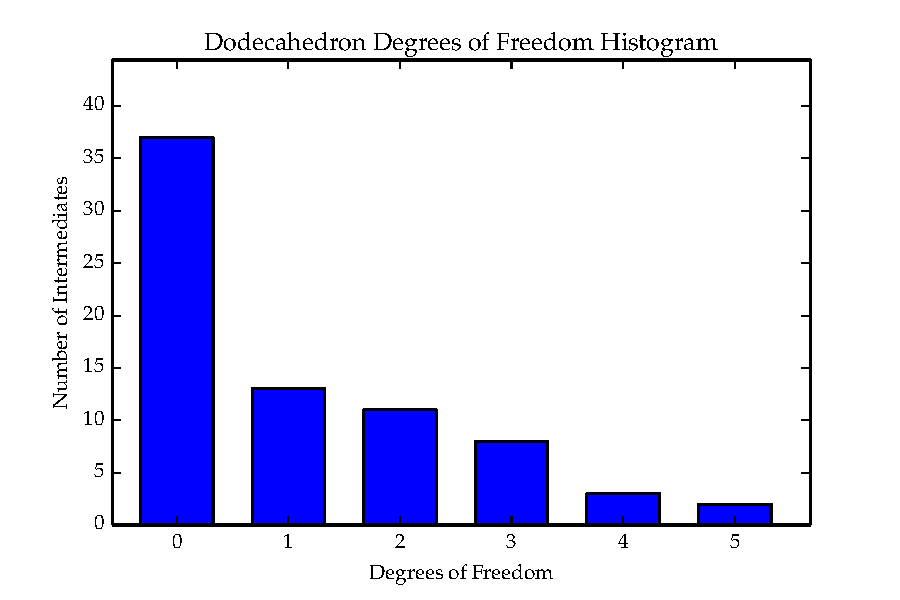
\includegraphics{dodecahedron_dof_hist.pdf}
}
\end{frame}
%% -----------------------------------------------------------------------------
\begin{frame}{Degrees of Freedom: Dodecahedron II}
 % \centering
\scalebox{0.5}{
 % \centering
        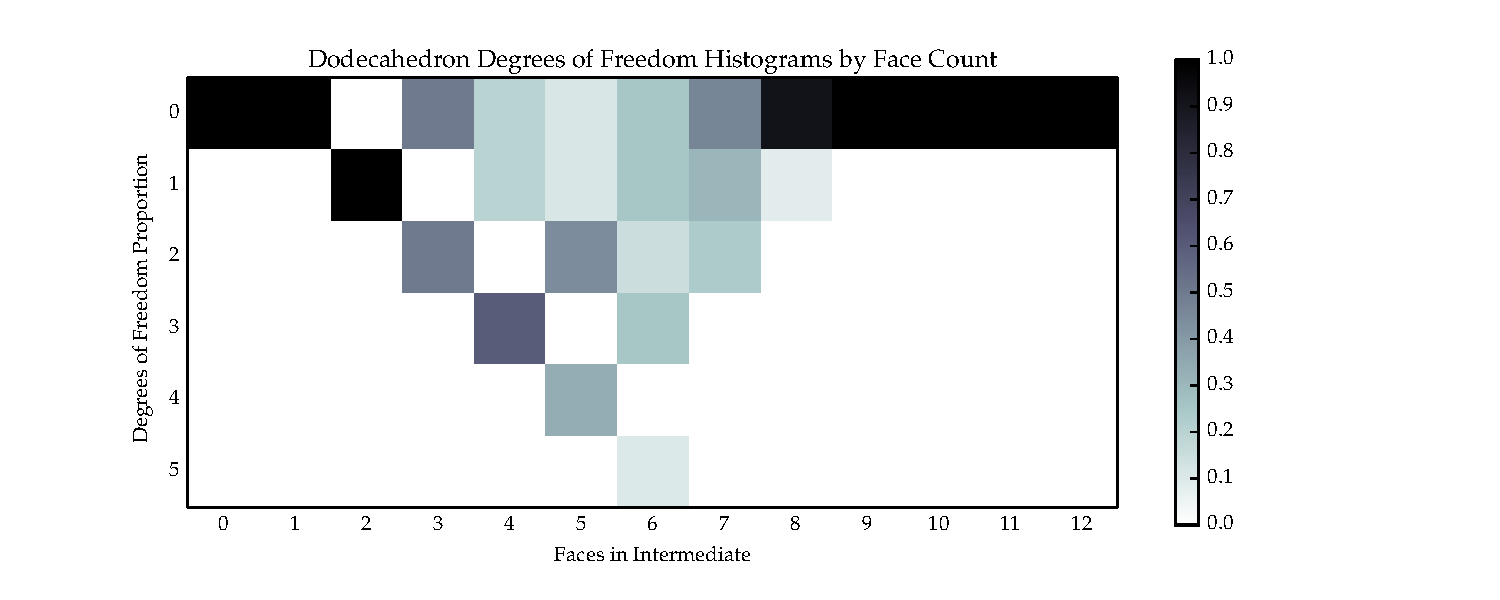
\includegraphics[trim=50 0 0 0, clip]{dodecahedron_dof_hist_facecount.pdf}
}
\end{frame}
%% -----------------------------------------------------------------------------
\begin{frame}{Degrees of Freedom: Icosahedron}
  \centering
\scalebox{0.6}{
        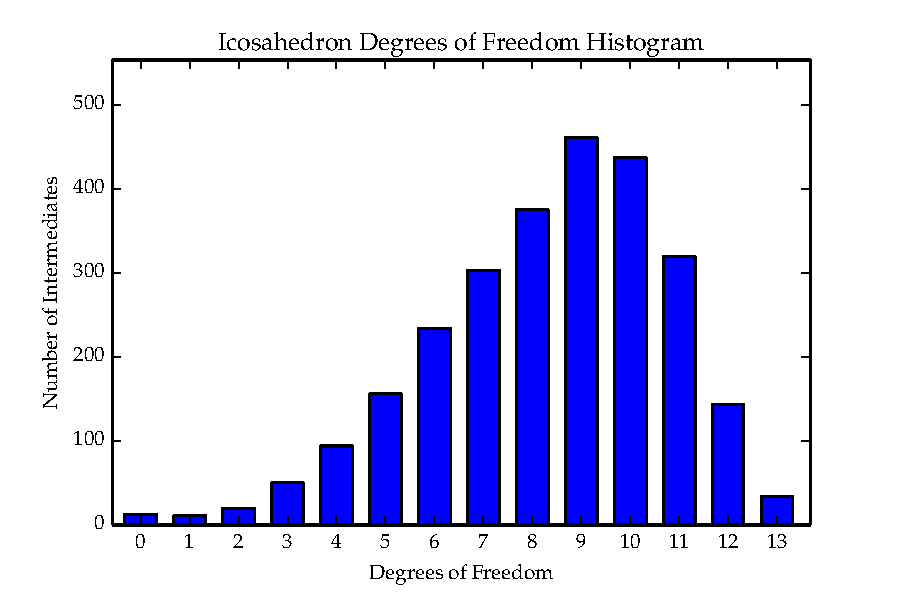
\includegraphics{icosahedron_dof_hist.pdf}
}
\end{frame}
%% -----------------------------------------------------------------------------
\begin{frame}{Degrees of Freedom: Icosahedron II}
  \centering
\scalebox{0.55}{
  %\begin{left}
        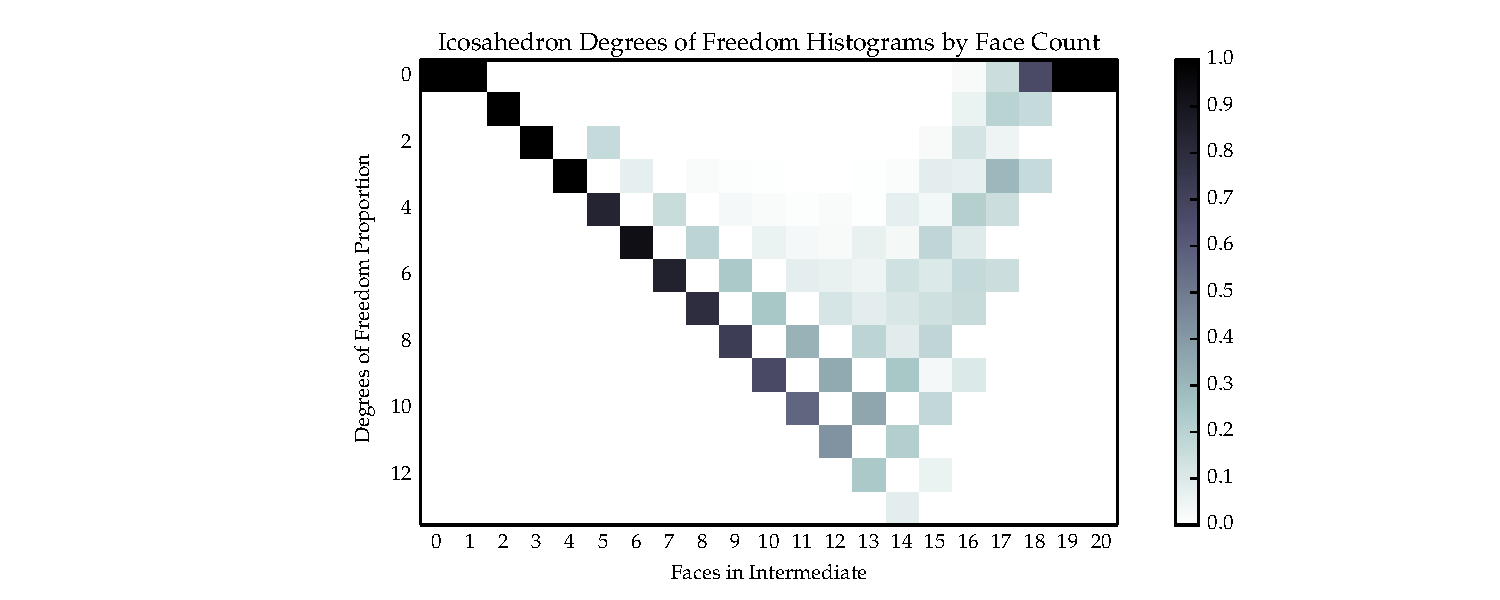
\includegraphics[trim=150 0 100 0, clip]{icosahedron_dof_hist_facecount.pdf}
  %     \end{left}
}
\end{frame}
%%% -----------------------------------------------------------------------------
%\begin{frame}{Degrees of Freedom by Number of Faces}
%add second hist
%  \centering
%    \scalebox{0.4}{
%      \begin{figure}
%        \centering
%        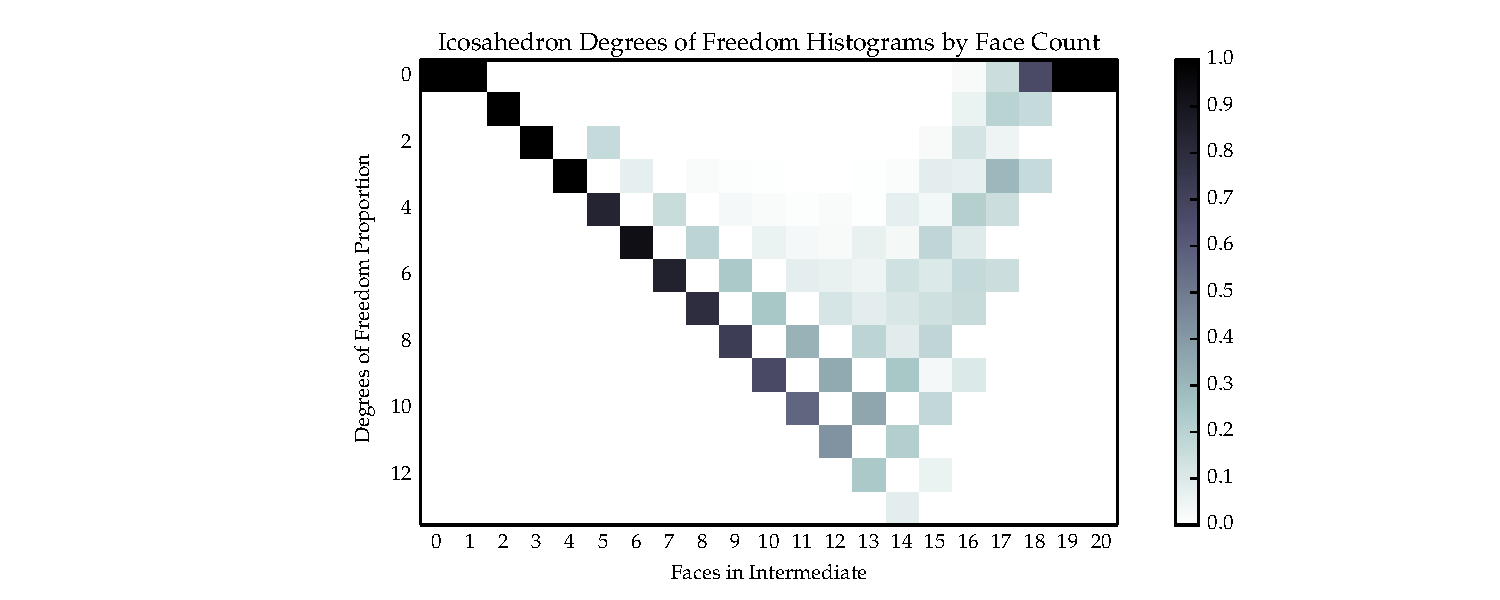
\includegraphics{icosahedron_dof_hist_facecount.pdf}
%       \end{figure}
%      }
%\end{frame}
%
% -----------------------------------------------------------------------------
% -----------------------------------------------------------------------------
\section{Reflected Brownian Motion}
% -----------------------------------------------------------------------------
\begin{frame}{Brownian Motion on Geometric Configuration Space}
\begin{itemize}
\item Brownian motion explores GCS 
\item Provides probabilistic framework for comparing different regions of the Geometric Configuration Space
\item Two stage random walk scheme
\begin{itemize}
 \item Take random step in tangent space $\mathcal{T}_z\mathcal{M}$
  \item Project new point back to $\mathcal{M}$
\end{itemize}
\end{itemize}
\end{frame}
% -----------------------------------------------------------------------------
\begin{frame}{Tangent Space}
\begin{itemize}
\item Use Jacobian of $c$: $C(z) \in \mathbbm{R}^{m\times n}$
\item $\mathcal{T}_z\mathcal{M} \doteq \left\{w \in \mathbbm{R}^n : C\left(z\right)w = 0\right\}$ 
\item Computation:
\begin{itemize}
\item Draw $B \in \mathbbm{R}^{n\times (n-m)}$ uniformly in $(0,1)$ at random.
\item Set $A = [C^T(z) B] \in \mathbbm{R}^{n\times n}$
\item Take the QR decomposition $A = [Q^{(1)} Q^{(2)}]R$
\item $Q^{(2)}$ orthonormal basis for $\mathcal{T}_z\mathcal{M}$ 
\end{itemize}
\end{itemize}
\end{frame}
% -----------------------------------------------------------------------------
\begin{frame}{Excluding Trivial Degrees of Freedom}
\begin{itemize}
\item Fix translations by imposing aditional constraints on center of mass.
\item Find bases $W \in \mathbbm{R}^{n\times 3}$ that correspond to rotation directions.
\item Use $A = [C^T(z) W \tilde{B}]$ where $\tilde{B} \in \mathbbm{R}^{n\times (n-m-3)}
\item $A = [Q^{(1)} Q^{(2)}_W Q^{(2)}_{\tilde{B}}]R$ gives basis 
\item Perform normal random walk and projection using $Q^{(2)}_{\tilde{B}}$
\item Rotate back to original frame of reference.
%\begin{align}
%  0 &= \sum_{i=1}^{n/3} v^i
%\end{align}
\end{itemize}
\end{frame}
%% -----------------------------------------------------------------------------
%\begin{frame}{Projection}
%Eqs
%\end{frame}
%% -----------------------------------------------------------------------------
%\begin{frame}{}
%MOVie
%\end{frame}
%% -----------------------------------------------------------------------------
\begin{frame}{Three Triangle Linkage}
add small T3 diagram
  \centering
    \scalebox{0.4}{
      \begin{figure}
        \centering
        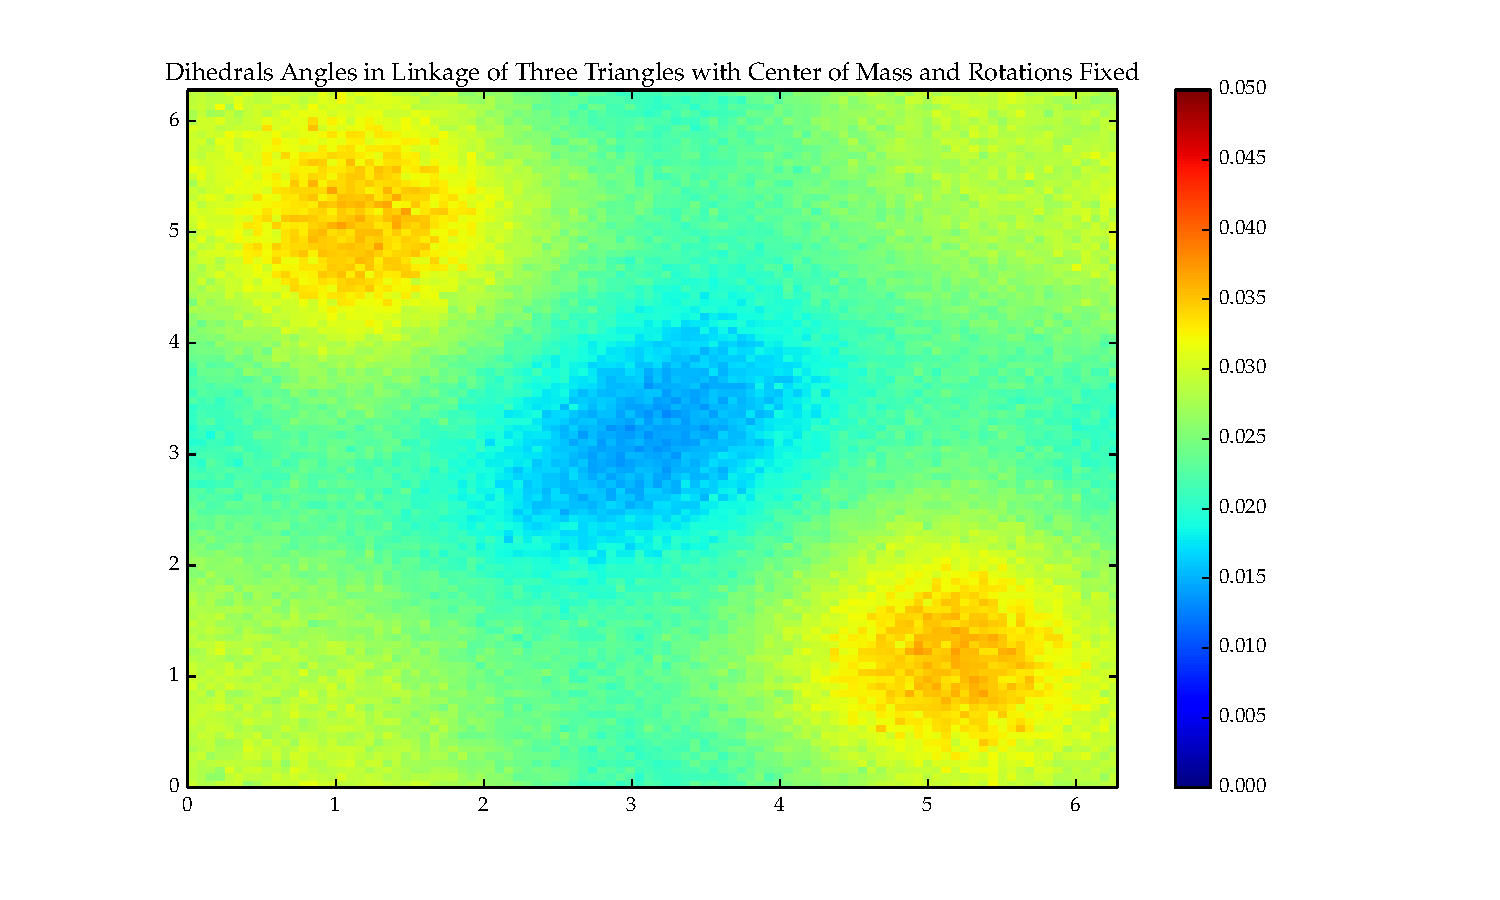
\includegraphics{T3_6_2D.pdf}
       \end{figure}
      }
\end{frame}
%% -----------------------------------------------------------------------------
%\begin{frame}{Example}
%MOVIE
%\end{frame}
% -----------------------------------------------------------------------------
\begin{frame}{Reflected Brownian Motion}
\begin{itemize}
\item Self-intersecting configurations are unphysical
\item Use reflected Brownian motion
\item At each iteration test for self-intersection.
\item Reject update if self-intersection found.
\end{itemize}
\end{frame}
% -----------------------------------------------------------------------------
\begin{frame}{Three Triangle Linkage}
  \centering
    \scalebox{0.4}{
      \begin{figure}
        \centering
        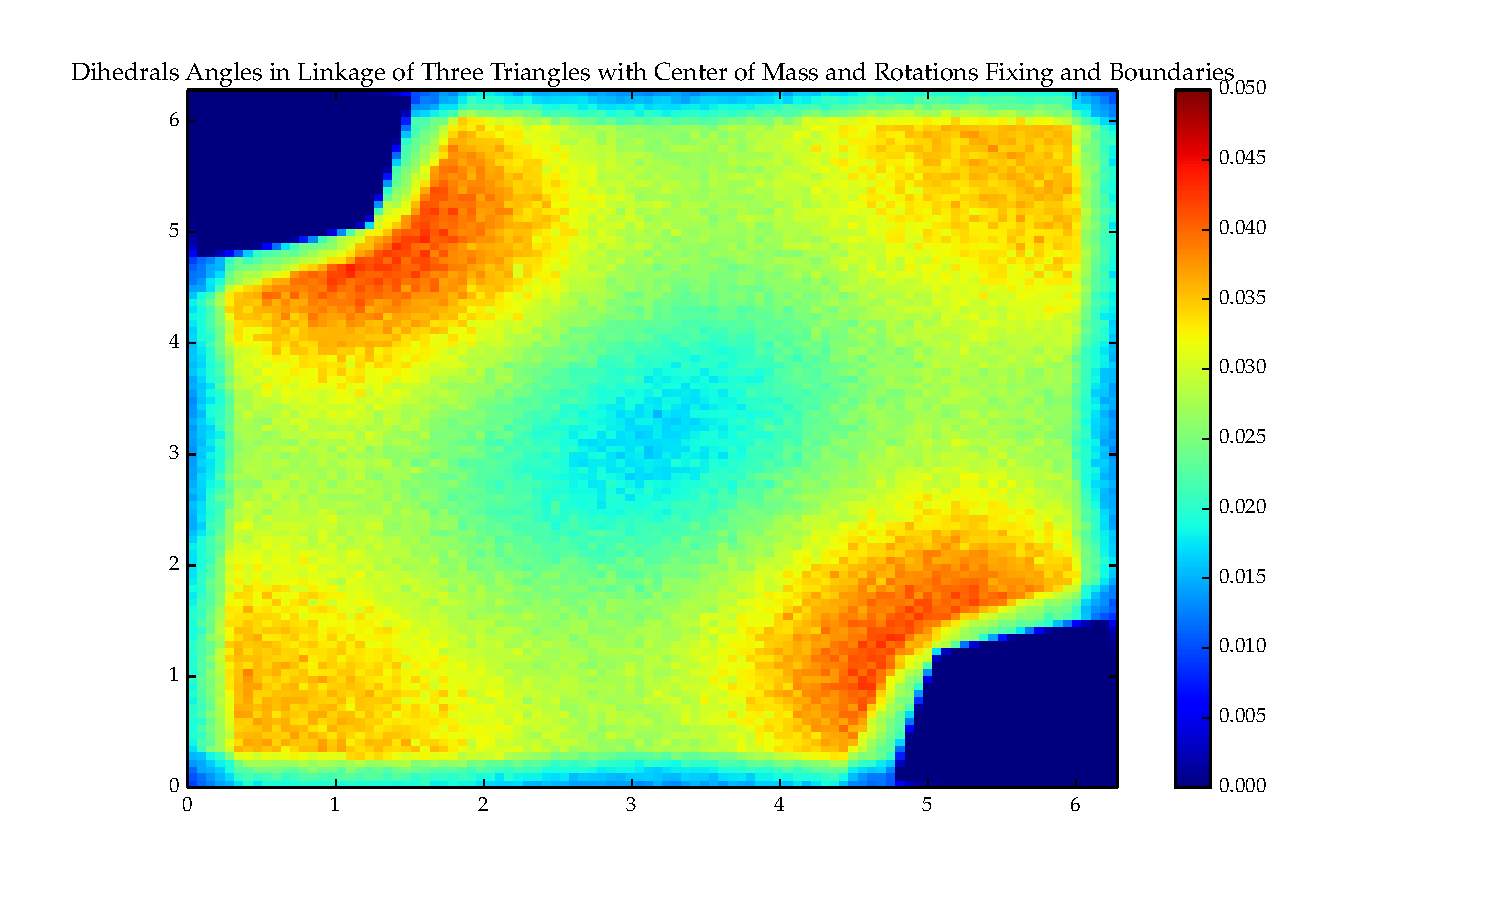
\includegraphics{T3_7_2D.pdf}
       \end{figure}
      }
\end{frame}
%% -----------------------------------------------------------------------------
%\begin{frame}{Example with Boundaries}
%MOVIE
%\end{frame}

% -----------------------------------------------------------------------------
% -----------------------------------------------------------------------------
\section{Results}
% -----------------------------------------------------------------------------
\begin{frame}{Finding Rates}
\end{frame}
% -----------------------------------------------------------------------------
\begin{frame}{Finding Barriers}
Use empirical rates to find Barrier heights. 
\begin{align}
\hat{Q}_{jk} &= Q^0_{jk} \\
	&= S_{jk}e^{\beta_0(E_{jk} - E_j)} \\
E_{jk} &= E_j-\frac{1}{\beta_0}\log\left(\hat{Q}_{jk}/S_{jk}\right) \\
Q_{jk} &= S_{jk}\left(\hat{Q}_{jk}/S_{jk}\right)^{\frac{\beta}{\beta_0}} \\
\end{align}

%$$Q_{jk} &= S_{jk}\left(\hat{Q}_{jk}/S_{jk}\right)^{\frac{\beta}{\beta_0}}$$

\end{frame}
% -----------------------------------------------------------------------------
\begin{frame}{Stationary Distribution}
  \centering
    \scalebox{0.4}{
      \begin{figure}
        \centering
        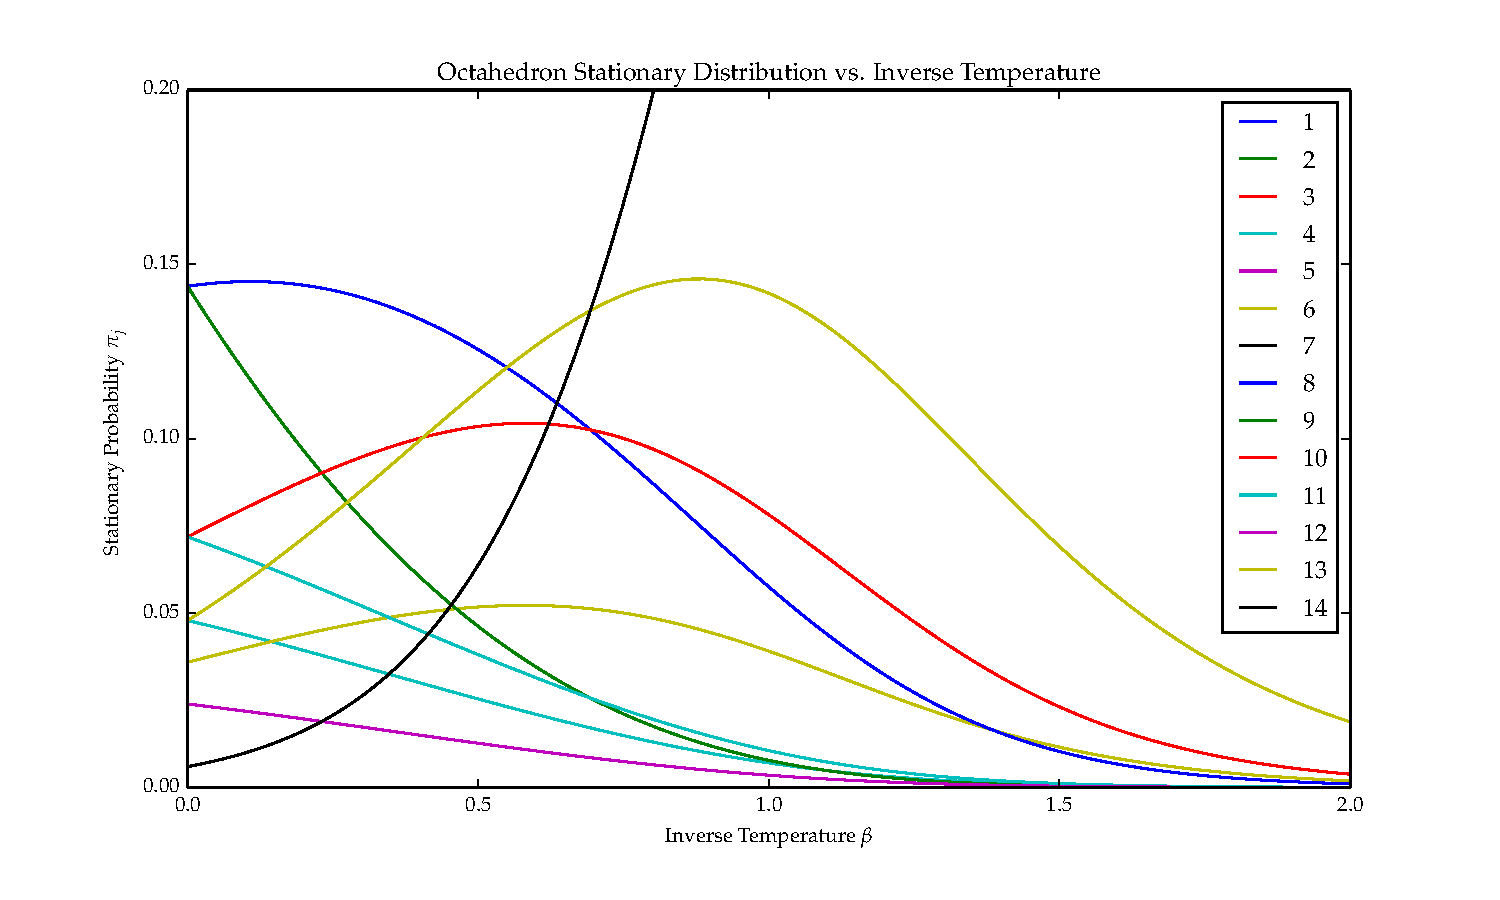
\includegraphics{octahedron_pi.pdf}
       \end{figure}
      }
\end{frame}
% -----------------------------------------------------------------------------
\begin{frame}{Finite Time Distribution}
  \centering
    \scalebox{0.4}{
      \begin{figure}
        \centering
        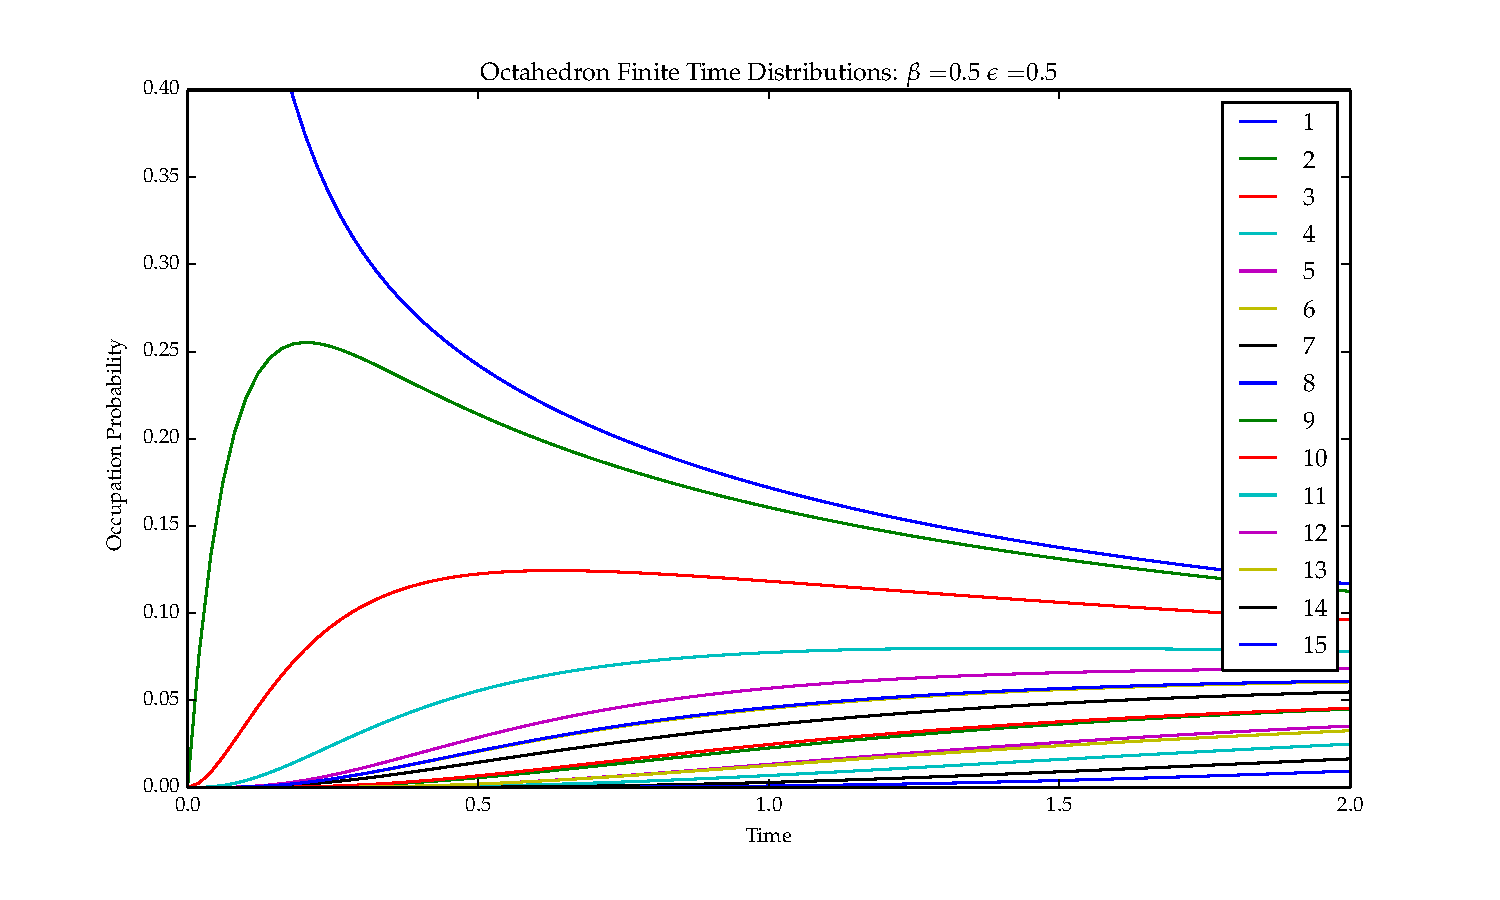
\includegraphics{octahedron_finite_dist.pdf}
       \end{figure}
      }
\end{frame}
% -----------------------------------------------------------------------------
\begin{frame}{Marvov Process on Octahedron CCS}
  \centering
    \scalebox{0.15}{
      \begin{figure}
        \centering
        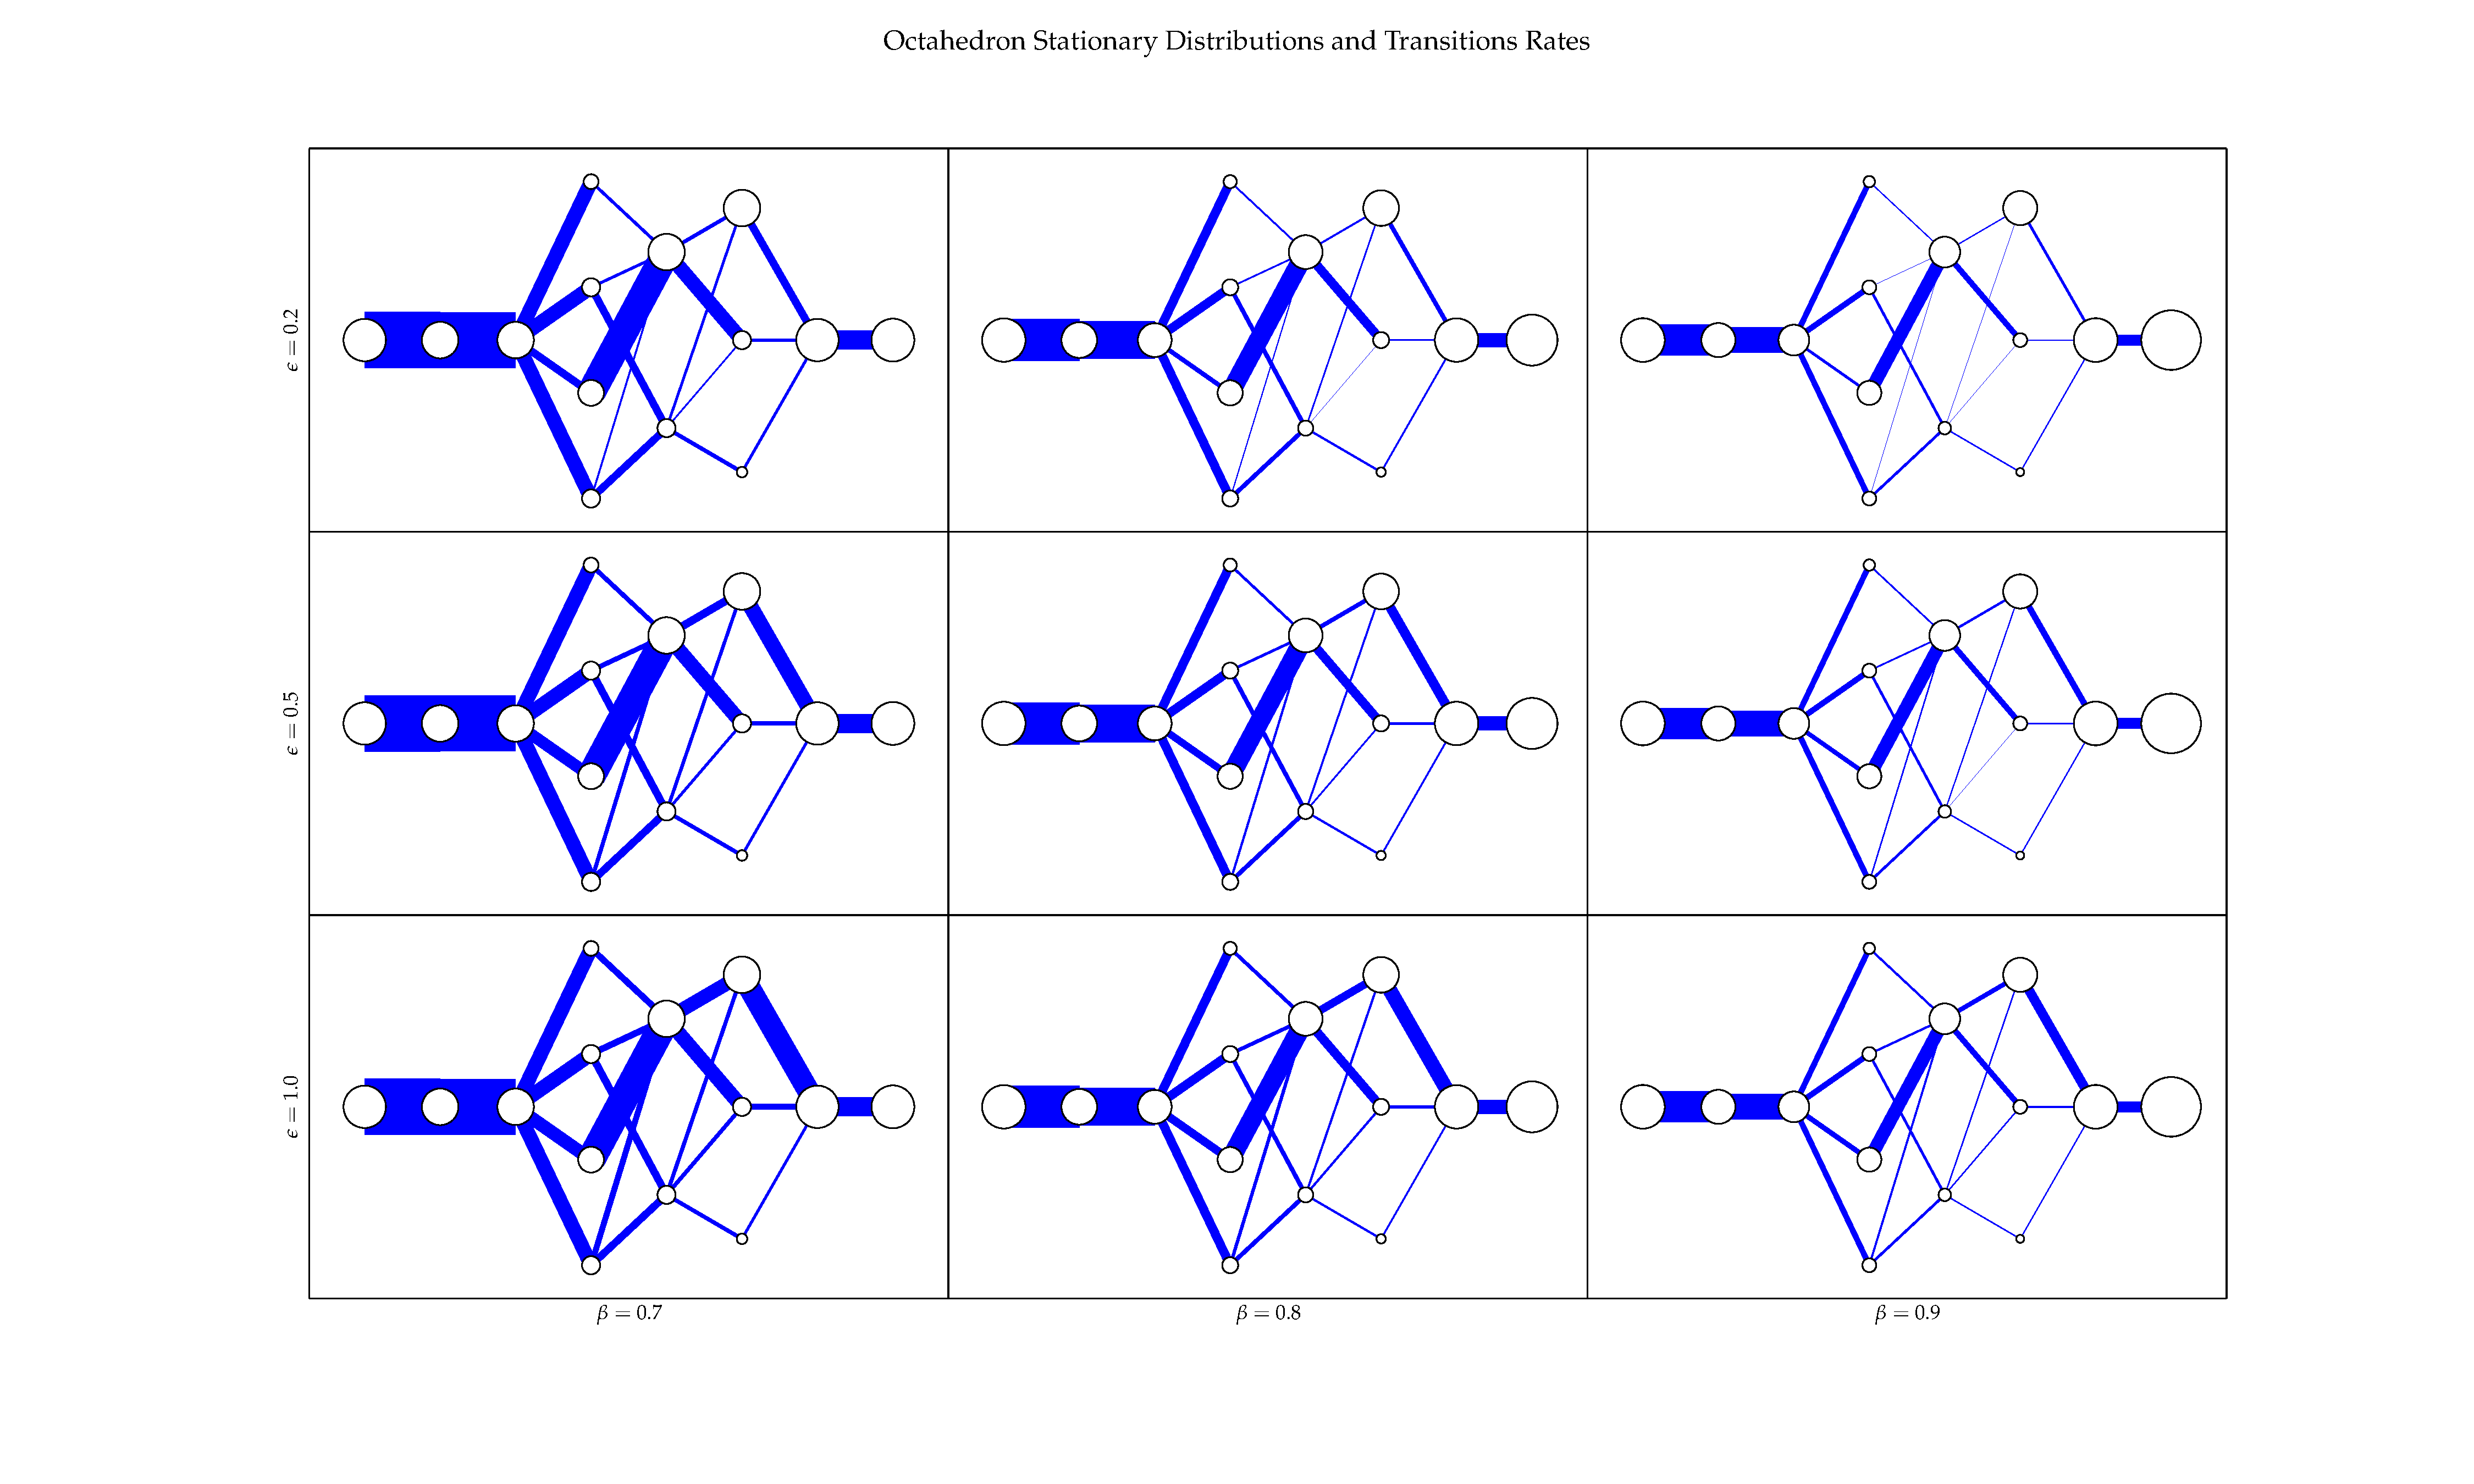
\includegraphics[trim = 100 0 0 0,clip]{octahedron_pi_Q_grid.pdf}
       \end{figure}
      }
\end{frame}
% -----------------------------------------------------------------------------
\begin{frame}{Expected Formation Times}
  \centering
    \scalebox{0.4}{
      \begin{figure}
        \centering
        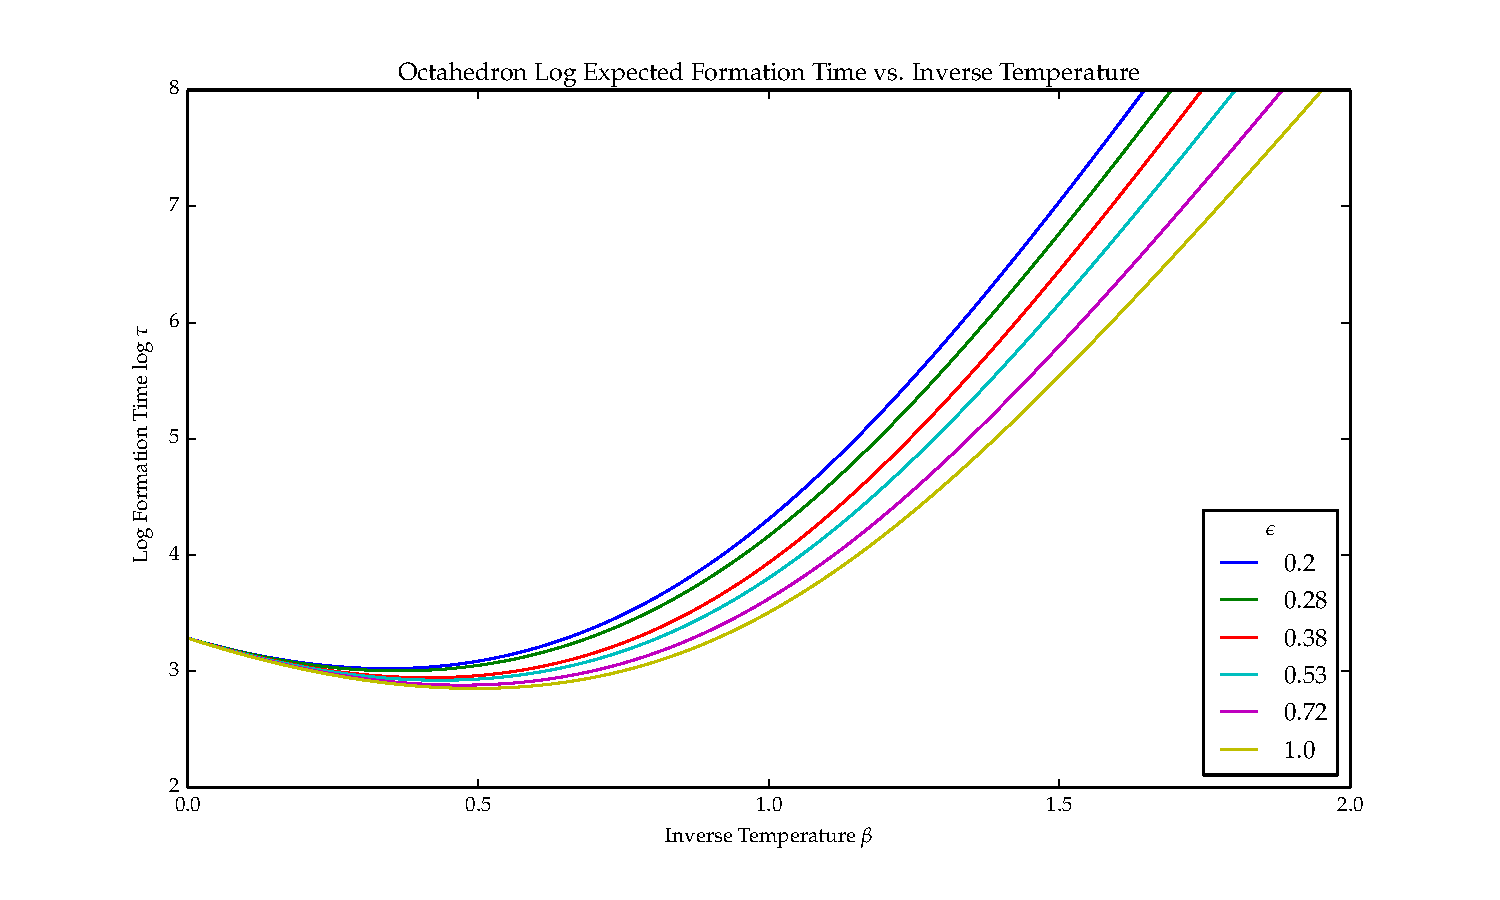
\includegraphics{octahedron_tau.pdf}
       \end{figure}
      }
\end{frame}
% -----------------------------------------------------------------------------






% -----------------------------------------------------------------------------
% -----------------------------------------------------------------------------
\section{Conclusions}
\begin{frame}{Summary}
\begin{itemize}
  \item Examined discrete geometric model for polyhedral construction
  \item Novel enumerative results
  \item Used Markov processes to compute formation statistics
\end{itemize}
\end{frame}
% -----------------------------------------------------------------------------
\begin{frame}{Acknowledgments}
\begin{itemize}
\item Thank you for inviting me to talk! 
\item Advisor: Govind Menon
\item Grants: NSF EFRI 10-22730, NSF EFRI 10-22638, NSF CMMI 1200241
\end{itemize}
\end{frame}


% -----------------------------------------------------------------------------
% -----------------------------------------------------------------------------
\section{Shellability}

%\subsection{Shellings}
\begin{frame}{Shellings and Shellability}
\begin{definition}
A \textbf{shelling} is a linear ordering $f_1, f_2, \dots f_N$ of a polyhedra's faces such that 
$$f_j \cap \left(\bigcup_{i=1}^{j-1}f_i\right)$$ is connected for each $j$.
\end{definition}
\begin{theorem}
$$\#(\text{shellings})&= \sum_{p \in \{\text{shellable paths}\}}|[x^{p_1}]|\prod_j^{|F|-1}S_{p_jp_{(j+1)}}$$
\end{theorem}
\end{frame}
%\subsection{Configuration Space Enumeration}
\begin{frame}{Shelling Enumeration}
\begin{figure}[ht]
\scalebox{0.6}{
%{\footnotesize
\centering
%\textbf{Building Game Enumerative Results for the Platonic Solids}
\begin{tabular}{ l | c | r}
Polyhedra Name & $|F|$ & Shellings \\
  \hline    
Tetrahedron                     & 4  	& 24 \\                         
Cube                            & 6  	& 480 \\                        
Octahedron                      & 8  	& 4,224\\                       
Dodecahedron                    & 12 	& 19,041,600 \\                 
Icosahedron                     & 20 	& 1,417,229,099,520 \\ \hline   
Truncated Tetrahedron           & 8     & 9,216 \\                      
Cuboctahedron                   & 14	& 113,055,744 \\                
Truncated Cube                  & 14	& 654,801,408 \\                
Truncated Octahedron            & 14	& 937,087,104 \\                
Rhombicuboctahedron             & 26	& 4,728,400,467,971,102,208 \\  
Truncated Cuboctahedron         & 26	& 688,499,026,944,479,645,952 \\ \hline
Triakis Tetrahedron             & 12    & 587,040\\                     
Rhombic Dodecahedron            & 12 	& 5,836,800\\                   
Triakis Octahedron              & 24	& 66,063,419,534,592 \\         
Tetrakis Hexahedron             & 24	& 1,389,323,257,015,296 \\      
Deltoidal Icositetrahedron      & 24	& 125,987,819,253,281,472\\     
Pentagonal Icositetrahedron     & 24	& 1,144,572,832,023,047,616 \\  
Rhombic Triacontahedron         & 30	& 15,574,782,555,813,226,074,240 \\
\end{tabular}
}
%\caption{Number of Shellings for the Platonic, Archimedean, and Catalan solids of up to 30 faces.}
\label{tab:Shellings}
\end{figure}
\end{frame}
% -----------------------------------------------------------------------------
\begin{frame}{Shelling Computation}
Dynamic programming relation! 
\begin{align}
a_{i,k} &\doteq \sum_{\substack{\text{shellable subpaths}:\\ p_1, \dots, p_k \\ x^{p_k} \in [x^i]}}|G.x^{p_1}|\prod_{j=1}^{k-1}S_{p_j p_{j+1}} \\  
&= \sum_{[x^\ell]:[x^\ell]\xrightarrow{shell}[x^i]} S_{\ell i} a_{\ell, k-1}
\end{align}
\end{frame}


\end{document}
% -----------------------------------------------------------------------------
% -----------------------------------------------------------------------------
% -----------------------------------------------------------------------------
% -----------------------------------------------------------------------------
% -----------------------------------------------------------------------------
\section{Introduction}
\subsection{Cracked Pots -- an uncharted field}
\begin{frame}{Why study Psychoceramics?}
  \begin{itemize}
    \item Plenty of subjects available for study
    \item Bright Job Prospects
    \item Ample Funding (Josiah S. Carberry Fund)
  \end{itemize}
\end{frame}
\begin{frame}{Past Work}
  Work done by JSC:
  \pause
  \begin{itemize}
    \item<2-> Archaic Greek Architectural Revetments in Connection with Ionian Philology
    \item<3-> Another Catullus to Another Lesbia
  \end{itemize}
  \pause[4]
  Work done by Others:
  \begin{itemize}
    \item<5-> Nothing
  \end{itemize}
  
\end{frame}
% -----------------------------------------------------------------------------
\section{Conclusions}
\subsection{Additional Aspects}
\begin{frame}{Questions and Answers}
  More Questions?

  \begin{itemize}
    \item Browse \url{http://tinyurl.com/43dwrt}.
    \item Contact my assistant Truman Grayson.
  \end{itemize}
  
\end{frame}
% -----------------------------------------------------------------------------


